\chapter{Más allá de lo básico}
\label{cha:no_tan_basico}



Ahora que sabemos escribir texto y darle formato, e incluir imágenes, tablas, y ecuaciones, es tiempo de entrar en aspectos no tan básicos de \LaTeX{} que mejorarán la calidad final de nuestro documento o nos ayudarán a ser más eficientes al momento de escribir la tesis.

Comenzamos con entornos útiles, mismos que ya se han utilizado a lo largo del libro, para luego conocer un poco más del preámbulo para la modificación de parámetros globales, así como la definición de nuevas instrucciones.



\section{Citas}
\label{sec:citas}



Me refiero a ``cita'' en la siguiente acepción:

\begin{displayquote}
Reproducción de las palabras dichas o escritas por alguien con el fin de apoyar o confirmar algo que se dice\footnote{Tercer definición provista por Google, en \href{https://www.google.com/search?q=definir+cita}{https://www.google.com/search?q=definir+cita}.}.
\end{displayquote}

\noindent y no en el sentido de... bueno, concertar una reunión romántica con una persona de interés (que, por inclusión, ya no se hace referencia a ``persona del sexo opuesto'').

Por ejemplo, la definición anterior es una cita hecha en el entorno \texttt{displayquote}, que requiere del paquete \texttt{csquotes}. Es decir, el código necesario fue:

\begin{lstlisting}[style=latex]
% Agregar el siguiente paquete en el preámbulo:
\usepackage{csquotes} % Mostrar citas de manera bonita, con sangrado.

\begin{displayquote}
Reproducción de las palabras dichas o escritas por alguien con el fin de apoyar o confirmar algo que se dice.
\end{displayquote}
\end{lstlisting}



\section{Columnas con \texttt{multicol}}
\label{sec:columnas_multicol}



En caso de querer $n$ columnas de la misma anchura se puede utilizar el entorno \texttt{multicols}, el cual viene en un paquete casi con el mismo nombre: \texttt{multicol}. Las siguientes dos columnas están hechas gracias a un entorno \texttt{multicols}:

\lstrulet\vspace{-9mm}\begin{multicols}{2}
Esta es la columna izquierda de un entorno \texttt{multicols}. El código base para este tipo de entornos se muestra en la columna derecha: el único parámetro obligatorio del entorno \texttt{multicols} es el número de columnas. Cada columna puede terminar de dos formas. La primera, de forma automática, dejando que \LaTeX{} divida el contenido lo más equitativamente posible. La segunda, de manera manual, utilizando la instrucción |\columnbreak| para terminar la columna actual.

\begin{lstlisting}[style=latex,frame={}]
\begin{multicols}{num de columnas}
Contenido de la primera columna.

\columnbreak

Contenido de la segunda columna.

\columnbreak

   .
   .

Contenido de la n columna...
\end{multicols}
\end{lstlisting}
\end{multicols}\vspace{-6mm}\lstruleb

No obstante, si usamos más |\columnbreak| que el número de columnas establecido no se generará un error: el resultado será contenido mal colocado en las páginas. Lo que sí genera un error es olvidar el único parámetro obligatorio del entorno, que nos obsequia el siguiente texto de error:

\begin{lstlisting}[style=errores]
Missing number, treated as zero. [E]
\end{lstlisting}



\section{Columnas con \texttt{minipage}}
\label{sec:columnas_minipage}



El problema con el entorno \texttt{multicols} es que hace que cada columna tenga la misma anchura, dada por la siguiente fórmula \cite{bib:multicol_multirow}:

\[
\mbox{anchura} = \frac{\mbox{\codigo{linewidth}} - (\mbox{cantidad de columnas} - 1) \times \mbox{separación entre columnas}}{\mbox{cantidad de columnas}}
\]

Si queremos columnas asimétricas, alguna de diferente ancho que las demás, es necesario hacer uso del entorno \texttt{minipage}, mismo que ya utilizamos en la sección \ref{sec:ecuaciones_lado_a_lado} para colocar ecuaciones lado a lado.

Al contrario que \texttt{multicols}, donde un entorno genera las $n$ columnas, para hacer columnas con \texttt{minipage} requerimos un entorno por columna, cada uno con su longitud determinada, y nosotros somos responsables de dar con el 100\% del ancho.

\noindent\begin{minipage}{0.58\linewidth}
Por ejemplo, esta columna tiene un ancho del 58\% del ancho de línea, mientras que el código del lado derecho abarca el 42\% restante. No obstante, no se puede distinguir muy bien dónde acaba la primera columna y empieza la segunda.
\end{minipage}
\begin{minipage}{0.42\linewidth}
\begin{lstlisting}[style=latex,frame={}]
\begin{minipage}{0.58\linewidth}
Contenido en texto.
\end{minipage}
\begin{minipage}{0.42\linewidth}
Código del texto.
\end{minipage}
\end{lstlisting}
\end{minipage}

\begin{minipage}{0.20\linewidth}
Otro problema de este entorno es que, si no usas |\noindent|...
\end{minipage}
\begin{minipage}{0.45\linewidth}\vspace{2pt}
toda la línea de entornos aparece con la indentación, lo que hace que las columnas sobresalgan del lado derecho, como en este ilegible ejemplo.
\end{minipage}
\begin{minipage}{0.35\linewidth}
Por lo tanto, hay que remover la indentación antes del primer \texttt{minipage} para evitar este desbordamiento.
\end{minipage}

\vspace{10pt}
Si no pudiste leer lo anterior, te entiendo. El entorno \texttt{minipage} no se separa de manera vertical del párrafo anterior, y tampoco coloca espacios entre columnas. Las cuatro líneas que sobresalen del margen derecho gracias a la indentación pertenecen a tres columnas, de longitudes de 20\%, 45\%, y 35\% de la línea (sabiendo esto, ya puedes leerlas).

Entonces, al utilizar \texttt{minipage} debes tener en cuenta esos tres detalles:
\begin{enumerate}
	\item La indentación hace que el margen izquierdo esté desplazado, lo que provoca un margen derecho sobresaliente. Es necesario removerla con un |\noindent|.
	\item No hay espacio vertical antes o después de un \texttt{minipage}. Si todo el contenido aparece sin separación, se puede agregar manualmente espacio vertical mediante |\vspace{10pt}|, o cualquier unidad y cantidad que parezca pertinente.
	\item Hay que considerar la división entre columnas de manera manual, lo que se puede realizar con \texttt{minipage} adicionales.
\end{enumerate}

\vspace{-3mm}\lstrulet
\noindent\begin{minipage}{0.02\linewidth}
1 2 3 4 5 6 7 8 9
\end{minipage}
\begin{minipage}{0.01\linewidth}
\end{minipage}
\begin{minipage}{0.47\linewidth}
La numeración a la derecha es un \texttt{minipage} del 2\% de la línea, mientras que el código ocupa el 46\%. Aunque esta columna de texto bien podría ocupar el 52\% restante, se optó por hacer columnas para separar visualmente el contenido, del 1\% a la izquierda, del 3\% a la derecha. El código de las columnas se muestra en la columna derecha.
\end{minipage}
\begin{minipage}{0.04\linewidth}
\end{minipage}
\begin{minipage}{0.46\linewidth}
\begin{lstlisting}[style=latex,frame={}]
\begin{minipage}{0.02\linewidth}
1 2 3 4 5 6 7 8 9
\end{minipage}
\begin{minipage}{0.01\linewidth}
\end{minipage}
\begin{minipage}{0.47\linewidth}
Columna de texto.
\end{minipage}
\begin{minipage}{0.04\linewidth}
\end{minipage}
\begin{minipage}{0.46\linewidth}
\end{lstlisting}
\end{minipage}
\newline\lstruleb

\vspace{5pt}
Para terminar esta sección, este párrafo se muestra visualmente separado del conjunto de columnas anterior gracias a un |\vspace{5pt}|.


\section{El preámbulo}
\label{sec:preambulo}



A lo largo de esta obra se ha hecho solo una cosa en el preámbulo: agregar, agregar, y volver a agregar paquetes. No obstante, sus funciones van más allá: es donde se dan todas las instrucciones de cómo se debe crear el documento.

¿Por qué en el preámbulo? Porque es donde \LaTeX{} toma las decisiones globales, aquellas que afectarán todo el documento. Por ejemplo, en el preámbulo es donde se define el tipo de documento (\texttt{article}, \texttt{book}, \texttt{report}, entre otros) mediante la instrucción |\documentclass|.

Esa sola instrucción cambia cómo se crea el documento, desde la primera página: el \texttt{article} inicia el contenido de su primera sección inmediatamente bajo el título y autor, mientras que el \texttt{book} y \texttt{report} tienen una portada, dejando el contenido para después. Además, \texttt{book} y \texttt{report} son diferentes porque la clase \texttt{book} se encarga de que cada capítulo comience en una página impar (página a la derecha de un libro físico abierto). Estas decisiones las tiene que saber \LaTeX{} de antemano para saber donde introducir páginas en blanco, por ejemplo.

Otra decisión global se tomó al agregar el paquete \texttt{babel}, con la opción de \texttt{mexico}. Lo que esta instrucción le dijo a \LaTeX{} fue algo como ``usa las reglas de separación de palabras del idioma español, y a los entornos \texttt{table} los llamas \emph{tabla}''.

Pero no todos los paquetes agregados impactan visualmente a nuestro documento. Algunos paquetes, como \texttt{csquotes}, agregan instrucciones para darnos más entornos con los cuales trabajar, pero no pasa nada si no los usamos.

Si hasta este momento hemos definido al preámbulo como ``el lugar ese donde se agregan los paquetes'', es momento de dar una definición un poco más completa:

\begin{displayquote}
El preámbulo es el espacio previo a la instrucción |\begin{document}| donde se añaden paquetes para extender la funcionalidad de \LaTeX{} y se realizan diversas configuraciones que pueden afectar todo el documento, según nuestras necesidades.
\end{displayquote}

Estas configuraciones pueden ser modificación de parámetros de ciertos paquetes, redefinición de instrucciones, o creación de nuevas. Antes de ver qué se puede hacer en este espacio, creamos un nuevo documento adicional que será llamado \texttt{package-conf.tex}, o como quieras llamarlo, donde irán todas las instrucciones que le queramos dar a \LaTeX{}. Sí, la configuración en el preámbulo puede convertirse en algo monstruoso, así que es mejor separarlo de una buena vez.

Agregar un archivo para configuración implica un cambio en el archivo principal, como se muestra en el listado \ref{lst:preambulo}. En la línea 7 se muestra la inclusión del archivo \texttt{package-conf.tex} (recuerda que la extensión no se coloca en la instrucción |\input|), mismo que debe ir después de la declaración de todos los paquetes, y antes de iniciar el entorno \texttt{document}.

\begin{lstlisting}[style=latex,numbers=left,caption={Estructura de archivos para incluir configuración en el preámbulo.},label=lst:preambulo,
linebackgroundcolor={%
	\ifnum \value{lstnumber} =  7 \color{codigo_linea_resaltada}
	\else \color{codigo_fondo}
	\fi % Tantos \fi como líneas subrayadas.
}]
\documentclass[12pt]{report}

\usepackage[utf8]{inputenc}
\usepackage[spanish,mexico]{babel}
% \usepackage{Más paquetes...}

% === División de palabras ====================================================
\hyphenation{el-e-ct-roenc-ef-al-og-raf-ista}

%%%%%%%%%%%%%%%%%%%%%%%%%%%%%%%%%%%%%%%%%%%%%%%%%%%%%%%%%%%%%%%%%%%%%%%%%%%%%%%
%%%%% Definición de constantes %%%%%%%%%%%%%%%%%%%%%%%%%%%%%%%%%%%%%%%%%%%%%%%%
%%%%%%%%%%%%%%%%%%%%%%%%%%%%%%%%%%%%%%%%%%%%%%%%%%%%%%%%%%%%%%%%%%%%%%%%%%%%%%%
% Las constantes aquí definidas se usan en más de una instrucción y, para evitar
% cambiar todas las instancias, mejor se declaran una vez para afectar todos los
% lugares donde se tengan que utilizar.

\newcommand{\espacioleyenda}{2pt} % Espacio entre leyenda y figuras, listados.

%%%%%%%%%%%%%%%%%%%%%%%%%%%%%%%%%%%%%%%%%%%%%%%%%%%%%%%%%%%%%%%%%%%%%%%%%%%%%%%
%%%%% Definición de colores usados en el documento (requiere xcolor) %%%%%%%%%%
%%%%%%%%%%%%%%%%%%%%%%%%%%%%%%%%%%%%%%%%%%%%%%%%%%%%%%%%%%%%%%%%%%%%%%%%%%%%%%%

% Definiendo un color en base a otros requiere \colorlet, no \definecolor.
%     https://tex.stackexchange.com/a/34913
%     https://texblog.org/2015/12/08/custom-colors-in-latex/
% Colores de prueba (amarrillo, verde limón, claro que sí).
\colorlet{ColorBase}{DeepPink}
\colorlet{Prueba1}{Gold}
\colorlet{Prueba2}{LimeGreen}
% Colores de la portada.
\colorlet{FondoPortada}{ColorBase!40!Black}
\colorlet{TextoPortada}{White}
\colorlet{FondoCodigoPortada}{ColorBase!15!Black}
% Colores de encabezado y pie de página.
\colorlet{PiePaginaNumeroPagina}{Black!85}
\colorlet{PiePaginaCapitulo}{Black!70}
% Colores del título de cada capítulo.
\colorlet{FondoCapitulo}{FondoPortada}
\colorlet{TextoCapitulo}{TextoPortada}
% Color de los enlaces.
\colorlet{Enlaces}{FondoPortada}
% Color del resaltado para instrucciones de LaTeX.
\definecolor{Resaltado}{rgb}{0.96, 0.96, 0.96}
% Colores para el código.
\colorlet{codigo_linea_margen}{ColorBase!50}
\colorlet{codigo_fondo}{White} % Cambiado a sin fondo para poder colocar \vdots sin blanco entre líneas.
\colorlet{codigo_numero_linea}{Black!45}
\colorlet{codigo_base}{Black!90}
\colorlet{codigo_cadena}{DarkGoldenrod!80}
\colorlet{codigo_comentarios}{Green!90!Black}
\colorlet{codigo_palabraclave}{Navy!70!Black} % Valor de impresión
% \colorlet{codigo_palabraclave}{Navy!80} % Valor de prueba para daltónicos.
\colorlet{codigo_identificador}{DarkRed!80}
\colorlet{codigo_linea_resaltada}{DarkGoldenrod!10}
% Color de las leyendas.
\colorlet{Leyendas}{Black!85}

%%%%%%%%%%%%%%%%%%%%%%%%%%%%%%%%%%%%%%%%%%%%%%%%%%%%%%%%%%%%%%%%%%%%%%%%%%%%%%%
%%%%% Configuración del paquete listings %%%%%%%%%%%%%%%%%%%%%%%%%%%%%%%%%%%%%%
%%%%%%%%%%%%%%%%%%%%%%%%%%%%%%%%%%%%%%%%%%%%%%%%%%%%%%%%%%%%%%%%%%%%%%%%%%%%%%%

% Cambio de los nombres utilizados a español.
\renewcommand{\lstlistingname}{Listado}
\renewcommand{\lstlistlistingname}{Índice de listados}
% Ajuste para aceptar caracteres del idioma español.
\lstset{
    literate= % Lista de símbolos en español que marcarían un error.
    {á}{{\'a}}1  {é}{{\'e}}1  {í}{{\'i}}1  {ó}{{\'o}}1  {ú}{{\'u}}1
    {Á}{{\'A}}1  {É}{{\'E}}1  {Í}{{\'I}}1  {Ó}{{\'O}}1  {Ú}{{\'U}}1
    {à}{{\`a}}1  {è}{{\`e}}1  {ì}{{\`i}}1  {ò}{{\`o}}1  {ù}{{\`u}}1
    {À}{{\`A}}1  {È}{{\'E}}1  {Ì}{{\`I}}1  {Ò}{{\`O}}1  {Ù}{{\`U}}1
    {ä}{{\"a}}1  {ë}{{\"e}}1  {ï}{{\"i}}1  {ö}{{\"o}}1  {ü}{{\"u}}1
    {Ä}{{\"A}}1  {Ë}{{\"E}}1  {Ï}{{\"I}}1  {Ö}{{\"O}}1  {Ü}{{\"U}}1
    {â}{{\^a}}1  {ê}{{\^e}}1  {î}{{\^i}}1  {ô}{{\^o}}1  {û}{{\^u}}1
    {Â}{{\^A}}1  {Ê}{{\^E}}1  {Î}{{\^I}}1  {Ô}{{\^O}}1  {Û}{{\^U}}1
    {œ}{{\oe}}1  {Œ}{{\OE}}1  {æ}{{\ae}}1  {Æ}{{\AE}}1  {ß}{{\ss}}1
    {ű}{{\H{u}}}1{Ű}{{\H{U}}}1{ő}{{\H{o}}}1{Ő}{{\H{O}}}1{¡}{{!`}}1
    {ç}{{\c c}}1 {Ç}{{\c C}}1 {ø}{{\o}}1   {å}{{\r a}}1 {Å}{{\r A}}1
    {€}{{\euro}}1{£}{{\pounds}}1           {«}{{\guillemotleft}}1
    {»}{{\guillemotright}}1   {ñ}{{\~n}}1  {Ñ}{{\~N}}1 {¿}{{?`}}1
}
% Opciones adicionales que afectarán a todos los listados del documento.
\lstset{
    language={},
    numbers=none,
    numbersep=5pt,
    numberstyle=\tiny\color{codigo_numero_linea},
    backgroundcolor=\color{codigo_fondo},
    basicstyle=\footnotesize\ttfamily\color{codigo_base},
    commentstyle=\itshape\color{codigo_comentarios},
    stringstyle=\color{codigo_cadena},
    keywordstyle=\bfseries\color{codigo_palabraclave},
    identifierstyle=\color{codigo_identificador},
    tabsize=4,
    captionpos=b,
    breaklines=true,
    frame=lines,
    rulecolor=\color{codigo_linea_margen},
    postbreak=\mbox{\textcolor{red}{$\hookrightarrow$}\space},
    upquote=true, % Tomado de https://tex.stackexchange.com/questions/166790/how-can-i-get-straight-double-quotes-in-listings
    abovecaptionskip=\espacioleyenda
    % Si se usa el escapechar | las tablas marcan error por el uso en alineación.
    % escapechar=|, %Tomado de https://tex.stackexchange.com/a/144171
}
% Estilo del código LaTeX utilizado exclusivamente en la portada.
\iflulu
\lstdefinestyle{portada}{
    language=[LaTeX]{TeX},
    frame={},
    basicstyle=\Large\ttfamily\color{TextoPortada},
    backgroundcolor={},
    keywordstyle=\color{ColorBase!50},
    identifierstyle=\color{TextoPortada},
    lineskip=20pt
}
\else
\lstdefinestyle{portada}{
    language=[LaTeX]{TeX},
    frame={},
    basicstyle=\LARGE\ttfamily\color{TextoPortada},
    backgroundcolor={},
    keywordstyle=\color{ColorBase!50},
    identifierstyle=\color{TextoPortada},
    lineskip=20pt
}
\fi
% Estilo del código LaTeX usado a lo largo del documento.
\lstdefinestyle{latex}{
    mathescape=true, % Usado para meter $\vdots$
    language=[LaTeX]{TeX},
    identifierstyle=\color{codigo_base},
    texcsstyle=*\bfseries\color{codigo_palabraclave},
    moretexcs={
    % Deberían estar pero no están.
    maketitle, part, subsection, subsubsection, paragraph, subparagraph,
    setlength, tableofcontents, addto, contentsname, listoffigures,
    listoftables, listfigurename, listtablename, guillemotright, guillemotright,
    % fontenc
    textquotedbl,
    % textcomp
    textquotesingle,
    % graphicx
    scalebox,graphicspath,includegraphics,
    % xcolor
    textcolor, colorlet, pagecolor, color, definecolor,
    % geometry
    geometry,
    % fancyhdr
    chaptermark, thechapter, chaptername,thepage,chapter,
    fancyhead, fancyfoot, fancypagestyle, headrule,
    % setspace
    doublespacing, onehalfspacing, setstretch,
    % caption.
    DeclareCaptionFont, captionsetup,
    % multirow
    multirow,
    % multicol
    columnbreak,
    % amssymb
    therefore, hdots,
    % mathtools
    prescript,
    % listings
    lstdefinestyle, lstset, lstinputlisting, lstlistlistingname, lstlistoflistings,
    % blindtext
    blindtext,
    % lipsum
    lipsum,
    % babel
    spanishtablename, captionsspanish,
    % titlesec
    titleformat, titleformat, titlespacing,
    % enumitem
    setlist,
    % hyperref
    hypersetup, url,
    % soulut8
    sethlcolor, hl,
    % Mis propios comandos.
    espacioleyenda, margenIzquierdo, margenDerecho,
    texttthl, instruccionlatex, hll
    }
}
\lstdefinestyle{latexi}{ % LaTeX inline
    style=latex,
    mathescape=false,
    basicstyle=\normalsize\ttfamily\color{codigo_base},
    columns=fixed,
    frame={},
}
% Texto rojo para resaltar errores.
\lstdefinestyle{errores}{
    basicstyle=\footnotesize\ttfamily\color{DarkRed!80!Black},
    commentstyle=\color{DarkRed!80!Black},
    keywordstyle=\color{DarkRed!80!Black},
    identifierstyle=\color{DarkRed!80!Black},
    mathescape=false, % Esto no puede ser true para este estilo, por el texto 'Missing $ inserted' (luego se marca un error)
}
% Texto amarillo para resaltar advertencias de compilación.
\lstdefinestyle{advertencias}{
    basicstyle=\footnotesize\ttfamily\color{DarkGoldenrod!70!Black},
    commentstyle=\color{DarkGoldenrod!70!Black},
    keywordstyle=\color{DarkGoldenrod!70!Black},
    identifierstyle=\color{DarkGoldenrod!70!Black},
    mathescape=false, % No marcar como true por uso de $.
}
% Definición del lenguaje BibTeX, para que tenga un poco de sintaxis.
\lstdefinelanguage{BibTeX}{
    keywords={%
        @tipo_de_fuente,@article,@book,@collectedbook,@conference,@electronic,@ieeetranbstctl,%
        @inbook,@incollectedbook,@incollection,@injournal,@inproceedings,%
        @manual,@mastersthesis,@masterthesis,@misc,@patent,@periodical,@phdthesis,@preamble,%
        @proceedings,@standard,@string,@techreport,@unpublished%
    },
    comment=[l]{\%},
    sensitive=false
}
% Definición del estilo BibTeX, para el capítulo de fuentes bibliográficas.
\lstdefinestyle{bibtex}{
    language=BibTeX,
    identifierstyle=\color{codigo_base},
    texcsstyle=*\bfseries\color{codigo_palabraclave},
    moretexcs={url}
}
% Permite usar las barras verticales para crear entornos en línea con el texto de estilo LaTeX.
%     Tomado de https://tex.stackexchange.com/questions/264293/cant-escape-curly-braces-in-lstinline
\lstMakeShortInline[style=latexi]|

%%%%%%%%%%%%%%%%%%%%%%%%%%%%%%%%%%%%%%%%%%%%%%%%%%%%%%%%%%%%%%%%%%%%%%%%%%%%%%%
%%%%% Configuración del paquete fancyhdr %%%%%%%%%%%%%%%%%%%%%%%%%%%%%%%%%%%%%%
%%%%%%%%%%%%%%%%%%%%%%%%%%%%%%%%%%%%%%%%%%%%%%%%%%%%%%%%%%%%%%%%%%%%%%%%%%%%%%%
\pagestyle{fancy}
\renewcommand{\chaptermark}[1]{\markboth{#1}{}}
\renewcommand{\headrule}{} % Remueve línea horizontal propia de fancyhdr.
\fancyhfoffset[L]{\margenAdicional}
\fancyhead[LE,CE,RE,LO,CO,RO]{} % Remover todo lo del encabezado.
\fancyfoot[LE,CE,RE,LO,CO,RO]{} % Remover todo lo del pie de página.
\fancyfoot[RO]{ % Para el pie de página de una página impar, a la derecha.
    \footnotesize % Todo el pie estará en este tamaño.
    \textcolor{PiePaginaCapitulo}{ % Color para nombre de capítulo.
        \leftmark % Imprimir el nombre del capítulo.
    } % Fin de cambio de color
    \kern10pt % Dejar un espacio de 10pt respecto a lo que siga.
    \textcolor{PiePaginaNumeroPagina}{ % Color para número de página.
        \textbf{\thepage} % Imprimir el número de página.
    } % Fin del otro cambio de color.
}
\fancyfoot[LE]{ % Para el pie de página de un página par, a la izquierda.
    \footnotesize % Todo el pie estará en este tamaño.
    \textcolor{PiePaginaNumeroPagina}{
        \textbf{\thepage} % Imprime el número de página.
    }
    \ifnum\value{chapter}>0 % \ifnum evita "Capítulo 0" en el índice.
        \kern10pt % Espacio entre número de página y otro texto.
        \textcolor{PiePaginaCapitulo}{
            \chaptername~\thechapter % Imprime "Capítulo" y número.
        }
    \fi % Fin del \ifnum.
}
\fancypagestyle{plain}{
    \fancyhead{} % Nada en el header.
    \renewcommand*{\headrule}{} % Eliminar la regla horizontal.
    \fancyfoot{} % Nada en el footer.
}

%%%%%%%%%%%%%%%%%%%%%%%%%%%%%%%%%%%%%%%%%%%%%%%%%%%%%%%%%%%%%%%%%%%%%%%%%%%%%%%
%%%%% Configuración del paquete fncychap %%%%%%%%%%%%%%%%%%%%%%%%%%%%%%%%%%%%%%
%%%%%%%%%%%%%%%%%%%%%%%%%%%%%%%%%%%%%%%%%%%%%%%%%%%%%%%%%%%%%%%%%%%%%%%%%%%%%%%

\renewcommand\DOCH{ % DOCH aplica para los capitulos con número y nombre.
\begin{adjustwidth}{-\margenIzquierdo-\margenAdicional}{-\margenDerecho}
    \nointerlineskip%
    \vspace{-1.625in}%
    \settowidth{\py}{\CNoV\thechapter}%
    \addtolength{\py}{\margenDerecho}%
    \addtolength{\py}{0.05in}%
    \fboxsep=0pt%
    \colorbox{FondoCapitulo}{\rule{0pt}{1.75in}\parbox[b]{1.01\paperwidth}{\hfill}}%
    \kern-\py\raise20pt%
    \hbox{\color{TextoCapitulo}\CNoV\thechapter}\\%
\end{adjustwidth}
}
\renewcommand\DOTI[1]{ % DOTI es para \chapter
\begin{adjustwidth}{-\margenIzquierdo-\margenAdicional}{0in}
    \nointerlineskip%
    \fboxsep=\myhi%
    \vskip-0.20in%
    \colorbox{FondoCapitulo}{\parbox[t]{\paperwidth}{\CTV\FmTi{\color{TextoCapitulo}#1}\kern\margenDerecho\kern0.055in}}\par\nobreak%
    \vskip-1ex%
    \colorbox{FondoCapitulo}{\rule{0pt}{10pt}\parbox[b]{\paperwidth}{\hfill}}%
    \vskip 30pt%
\end{adjustwidth}
}
\renewcommand\DOTIS[1]{ % DOTIS aplica para los capítulos sin número y sin nombre (\chapter*).
\begin{adjustwidth}{-\margenIzquierdo-\margenAdicional}{0in}
    \vspace{-1.85in}
    \fboxsep=0pt
    \colorbox{FondoCapitulo}{\rule{0pt}{120pt}\parbox[b]{1.01\paperwidth}{\hfill}}\\%
    \nointerlineskip%
    \fboxsep=\myhi%`
    \vskip-1ex%
    \colorbox{FondoCapitulo}{\parbox[t]{\paperwidth}{\CTV\FmTi{\color{TextoCapitulo}#1}\kern\margenDerecho}}\par\nobreak%
    \vskip-1ex%
    \colorbox{FondoCapitulo}{\rule{0pt}{10pt}\parbox[b]{\paperwidth}{\hfill}}%
    \vskip 30pt%
\end{adjustwidth}
}

%%%%%%%%%%%%%%%%%%%%%%%%%%%%%%%%%%%%%%%%%%%%%%%%%%%%%%%%%%%%%%%%%%%%%%%%%%%%%%%
%%%%% Ajustes de titlesec %%%%%%%%%%%%%%%%%%%%%%%%%%%%%%%%%%%%%%%%%%%%%%%%%%%%%
%%%%%%%%%%%%%%%%%%%%%%%%%%%%%%%%%%%%%%%%%%%%%%%%%%%%%%%%%%%%%%%%%%%%%%%%%%%%%%%

% Esta línea se activa en caso de no querer números en las secciones (usar en conjunto con secnumdepth)
% \titleformat{\section}{\normalfont\bfseries\Large}{}{0pt}{}{}
% Modifica el espacio entre el título y el texto que tiene debajo.
\titlespacing{\section}{-\margenAdicional}{*4}{*1.5}

% SE aplica una lógica similar para la subsección.
\titleformat*{\subsection}{\itshape\Large}
\titlespacing{\subsection}{0in}{*3}{*1.0}

%%%%%%%%%%%%%%%%%%%%%%%%%%%%%%%%%%%%%%%%%%%%%%%%%%%%%%%%%%%%%%%%%%%%%%%%%%%%%%%
%%%%% Configuración de otros paquetes %%%%%%%%%%%%%%%%%%%%%%%%%%%%%%%%%%%%%%%%%
%%%%%%%%%%%%%%%%%%%%%%%%%%%%%%%%%%%%%%%%%%%%%%%%%%%%%%%%%%%%%%%%%%%%%%%%%%%%%%%

% Configuración del enlaces (requiere hyperref).
\hypersetup{colorlinks, breaklinks, urlcolor=Enlaces, citecolor=Enlaces, linkcolor=Enlaces}

% Color del texto resaltado (requiere soulutf8).
% \sethlcolor{Resaltado} % Obtenido de https://tex.stackexchange.com/a/42964

% Configuración de las leyendas de figuras (requiere caption).
\DeclareCaptionFont{color_leyenda}{\color{Leyendas}}
\captionsetup{
    font={small,color_leyenda}, % Color y tamaño de la leyenda.
    skip=\espacioleyenda        % Espacio entre leyenda y figura. Default = 10pt.
}

% Ajuste del interlineado (requiere setspace).
\setstretch{1.1875}

% Elimina el espacio entre elementos de una lista (requiere enumitem).
\setlist{noitemsep}

%%%%%%%%%%%%%%%%%%%%%%%%%%%%%%%%%%%%%%%%%%%%%%%%%%%%%%%%%%%%%%%%%%%%%%%%%%%%%%%
%%%%% Otras configuraciones que afectan el comportamiento de LaTeX %%%%%%%%%%%%
%%%%%%%%%%%%%%%%%%%%%%%%%%%%%%%%%%%%%%%%%%%%%%%%%%%%%%%%%%%%%%%%%%%%%%%%%%%%%%%

% Longitud del sangrado de párrafos.
\setlength\parindent{0.25in}

% No numerar secciones (los mantenemos en el libro para dar apariencia de tesis, donde todo va numerado).
% \setcounter{secnumdepth}{0}
% Numerar capítulos y secciones solamente (pero no subsecciones y debajo).
\setcounter{secnumdepth}{1}

% Nombre de tabla de contenido.
\addto\captionsspanish{\renewcommand{\contentsname}{Contenido}}
% \setcounter{tocdepth}{1} % Capítulos y secciones en el índice.
\setcounter{tocdepth}{2} % Capítulos, secciones, y subsecciones en el índice.

% No "justificar" verticalmente (que LaTeX no busque que la última línea de todas las páginas quede donde mismo).
\raggedbottom

% Valores que afectan a cómo LaTeX maneja las líneas huérfanas (líneas que alcanzan a cruzar a otras páginas, solas).
\widowpenalty=10000
\clubpenalty=10000

%%%%%%%%%%%%%%%%%%%%%%%%%%%%%%%%%%%%%%%%%%%%%%%%%%%%%%%%%%%%%%%%%%%%%%%%%%%%%%%
%%%%% Nuevos comandos %%%%%%%%%%%%%%%%%%%%%%%%%%%%%%%%%%%%%%%%%%%%%%%%%%%%%%%%%
%%%%%%%%%%%%%%%%%%%%%%%%%%%%%%%%%%%%%%%%%%%%%%%%%%%%%%%%%%%%%%%%%%%%%%%%%%%%%%%

% Comando para encapsular texto que hace referencia a una opción de un menú de interfaz.
\newcommand{\opcionMenu}[1]{\emph{\texttt{#1}}}
% Puntos verticales a ser usados en los listados.
\newcommand{\puntitoscodigo}{\scalebox{0.80}{\vdots}}
% Parche para la doble diagonal en línea con el texto.
\newcommand{\diagonalesCodigo}{\textcolor{codigo_palabraclave}{\textbf{\texttt{\textbackslash\textbackslash}}}}
\newcommand{\codigo}[1]{\textcolor{codigo_palabraclave}{\textbf{\texttt{\textbackslash{}#1}}}}
\newcommand{\comentario}[1]{\textcolor{codigo_comentarios}{{\hypersetup{linkcolor=codigo_comentarios}\emph{\texttt{#1}}}}}
% Parte de la explicación de instrucciones.
\newcommand{\texttthl}[1]{\texttt{\hl{#1}}}
\newcommand{\ttlatex}[1]{\texttt{\textbackslash{}#1}}
\newcommand{\instruccionlatex}[1]{\texttthl{\textbackslash{}#1}}

\newcommand{\BibTeX}{\textsc{Bib}\TeX{}}
\newcommand{\BibLaTeX}{\textsc{Bib}\LaTeX{}}

\newcommand{\fuenteOverleaf}[1]{\footnote{Ejemplo en Overleaf, en \href{http://overleaf.ramoscarlos.com}{http://overleaf.ramoscarlos.com}, archivo \texttt{#1}.}}

% Comando para hacer capítulo sin numerar, pero que aparezca en el índice.
\newcommand\chap[1]{
    \cleardoublepage
    \phantomsection
    \addcontentsline{toc}{chapter}{#1}
    \chapter*{#1}
}

\newcommand{\lstrulet}{\noindent\textcolor{codigo_linea_margen}{\rule{\textwidth}{0.4pt}}\newline}
\newcommand{\lstruleb}{\noindent\textcolor{codigo_linea_margen}{\rule{\textwidth}{0.4pt}}}

\author{Carlos Ramos}

\begin{document}

% Portada y otras instrucciones previas a los capítulos...

\chapter{Introducción}
\label{cha:introduccion}



Este libro está diseñado con un público muy particular en mente, tal y como se establece en el título: estudiantes de ingeniería que deben escribir toda su tesis en este gran sistema de composición de textos que es \LaTeX{} (cuando lo leas en tu mente, que se escuche algo como \emph{leitec}, no como material de preservativos).

Por supuesto, al empezar a trabajar con \LaTeX{} hace años esos no eran los adjetivos que utilizaba para describir este sistema, y más bien lo definía como ``una herramienta tecnológica de tortura del siglo XX usada por la Inquisición Académica''.

Resulta que las imágenes no se insertaban al ser arrastradas al editor, y tampoco se quedaban donde yo les decía, ¿para qué servía el código entonces? Introducir caracteres en español era un horror, y los fragmentos de código que insertaba solo respetaban el alfabeto inglés, convirtiendo las letras acentuadas en símbolos horribles\footnote{Vale, no eran símbolos extraídos del \emph{Necronomicón}, pero me causaron pesadillas por mi ignorancia.}. Posiblemente, la mitad de mi tesis se fue en una pelea infructuosa en contra de \LaTeX.

Si tanta fue mi agonía, ¿por qué me empeñé tanto en usar \LaTeX{}  como sistema de composición de un documento tan extenso como lo fue mi tesis? Por una razón: era requisito, al menos en mi carrera (un requisito no compartido uniformemente en mi institución, lo que solo sirvió para incrementar mi frustración en aquellos ayeres).

Quizá esta es tu primera exposición a \LaTeX, y has comenzado de una manera similar a la mía: sabrá Dios qué es, sabrá Dios cómo se usa\footnote{Como este es un documento laico, esta es la única referencia a una deidad que verás aquí.}, pero un director de tesis anticuado desea que redactes en esta cosa compleja, que ni interfaz tiene, que parece más código que otra cosa, y que no sabes por qué tienes que utilizar si existe Word.

Lo bueno es que estás de suerte porque este libro lo escribí como respuesta a ``¿Qué hago si tengo que utilizar \LaTeX{} para escribir mi tesis y no sé dónde empezar?''
Mi objetivo es evitarte muchas de las frustraciones que yo sufrí durante la redacción de mi tesis mientras aprendía a utilizar \LaTeX{}. Pero he de advertirte: esta obra contiene algunas de mis vivencias como tesista y algunas opiniones personales, incluidas con el objetivo de hacer amena la lectura. Toma lo que te sirva, desecha lo que no.

Definido el tono del libro, comencemos con la teoría.



\section{¿Qué es?}
\label{sec:que_es}



Si no te preguntas qué es \LaTeX{}, haces bien, ¿para qué saber? Ah, cierto, requisitos que cumplir\footnote{Si estás aquí por gusto, eres de la inimaginable minoría. Igual será un placer ser tu guía.}. Comencemos definiendo lo que \emph{no es}. \LaTeX{} no es un sistema \emph{WYSIWYG} (lo que ves es lo que obtienes\footnote{Del inglés ``What You See Is What You Get''}) como lo es Microsoft Word, a pesar de que ya hay opciones que permiten generar un documento de \LaTeX{} en una interfaz algo similar. No obstante, sigue siendo mejor escribir el ``código'' que será el documento final.

Pero, ¿por qué? Con la existencia de procesadores de texto tan poderosos, con una interfaz amigable, ¿para qué molestarse en aprender a utilizar \LaTeX, que aparenta ser tan arcaico? ¿Por qué nadie se ha preocupado en hacer una interfaz para que \LaTeX{} sea tan \emph{WYSIWYG} como Word?

Esas respuestas solamente se puede obtener indagando en las características de \LaTeX{}, mismas que nos ayudarán a definir qué es.



\subsection{Contenido sobre formato}
\label{ssub:contenido_sobre_formato}



\LaTeX{} se centra en el contenido. Si sabes un poco de páginas web, podríamos decir que \LaTeX{} es el equivalente al HTML de una página en el sentido de que define la estructura de cómo se debe desplegar el documento. Extendiendo la analogía, el código HTML no se puede visualizar sin un navegador que lo interprete. De la misma forma, \LaTeX{} necesita al compilador para pasar de código a documento presentable.

Aún más, podríamos decir que el CSS, la parte de una página que hace que se vea bonita, equivale a configuraciones de \LaTeX{} en el preámbulo, mismas que nos permiten modificar la presentación del contenido sin cambiar nada, o casi nada, del código utilizado durante la redacción.

En otras palabras, al redactar en \LaTeX{} no nos preocuparemos por el formato, al menos no en primera instancia, y posiblemente ni en segunda, ni en tercera. Es decir, no es necesario pensar en cómo se ven los títulos, la numeración de páginas, si el texto va justificado, o qué fuente vamos a utilizar, mientras estemos en la fase de redacción.

Tanto así que este libro empieza de lleno con el contenido, con enfoque en lo que vas a escribir, explicando cómo hacer listas numeradas o sin numerar, cómo meter imágenes, tablas o código, pero no brinda detalles de cómo cambiar cuestiones de estilo. Porque, de nuevo, importa más el contenido que el formato.

Además, si vas a redactar una tesis para tu institución educativa, lo más probable es que ya tengas una plantilla la cual tienes que seguir, a pesar de que la consideres un crimen en contra de todo sentido de la estética. Requisitos son requisitos.

No puedo terminar esta sección sin enfatizar nuevamente: el formato no es el protagonista en \LaTeX{}, ocúpate de escribir. Al último trabajaremos con la apariencia.



\subsection{Instrucciones}
\label{ssub:instrucciones}



Aún no vemos cómo se ve el código de un documento realizado con \LaTeX, pero basta decir que se asemeja mucho a código de computadora, a cosas ininteligibles para seres mortales. Sí, suena a complicaciones innecesarias para realizar un documento que parece destinado a solo satisfacer el ego de unos cuantos.

No obstante, lo que distingue a \LaTeX{} es precisamente esta forma de trabajar, estas instrucciones que al final del día conforman el documento final, y que van mano a mano del punto anterior: el contenido va primero, antes que todo formato.

¿Y qué es una instrucción? Es una orden o comando que la computadora tomará para traducirla desde tu ``yo escribo contenido'' al producto final en PDF\footnote{Se puede realizar una conversión a otros formatos, pero eso escapa el alcance de este libro.} de ``computadora genera formato''. Podemos verlo en términos de la figura \ref{fig:esquema_latex}:

% Código obtenido de https://web.iit.edu/sites/web/files/departments/academic-affairs/graduate-academic-affairs/pdfs/figure-help1.pdf
\begin{figure}[ht!]
	\setlength{\unitlength}{3.5mm} % selección de unidad de medida.
\centering % La figura se centra
\begin{picture}(32, 5)  % ancho * alto
	% Las coordenadas del comando "put" son en base a la esquina inferior izquierda.
	\put(9,0.5){\framebox(14,4){Instrucciones en \LaTeX}}
	\put(1.5,2.5){\vector(1,0){7.5}}
	\put(23,2.5){\vector(1,0){7.5}}
	\put(1.5,3){Nuestro texto}
	\put(24,3) {PDF final}
\end{picture}
	\caption{Esquema de trabajo en \LaTeX.} % Leyenda de la figura.
	\label{fig:esquema_latex}
\end{figure}

Como ejemplo, para generar este libro solo pensé en este capítulo como ``Introducción''. Al momento de escribir, no sabía si sería ``Capítulo 1'', ``Capítulo I'', o solo diría ``1'', o si estaría numerado, siquiera.

No me preocupé de si estaría alineado a la derecha o a la izquierda, o el tamaño de la letra. Simplemente introduje el siguiente código (técnicamente, es más correcto decir ``la siguiente instrucción'' pero suena mejor de esta manera):

\begin{lstlisting}[style=latex]
\chapter{Introducción}
\end{lstlisting}

Y con eso me liberé de preocuparme por el formato. Sí, en algún momento el cómo regresó a perseguirme, pero no mientras estaba escribiendo e investigando.

De la misma forma, no deberás ocuparte del formato mientras estés en la fase de \st{generar resultados falsos y rellenar con mentiras para llegar a un m\'inimo de hojas} investigación, desarrollo, y documentación, sino hasta que tu asesor te diga que el contenido está bien aunque el formato no tanto.



\subsection{\TeX{} y \LaTeX{}}
\label{ssub:tex_latex}



En el punto anterior vimos que \LaTeX{} utiliza instrucciones para generar documentos. Pero, en realidad, \LaTeX{} no es otra cosa que \TeX{} con esteroides. ¿Qué significa ésto? ¿Acaso existen otras versiones? ¿Qué importa si es \LaTeX, \TeX, Lua\TeX, o sabrá que otra abominación con \TeX{} al final?

No es que importe mucho en sí la historia, pero un tío llamado Donald Knuth creó \TeX{} allá por 1978, con una licencia de código abierto. De ahí, otras personas empezaron a empalmar sus modificaciones y atajos, como más formas de estilizar texto, o para sus aplicaciones particulares de fórmulas, código, alfabetos, y más.

Entonces, \LaTeX{} viene a ser la forma más popular de \TeX{} que existe, con macros o instrucciones agregadas por muchísima gente a lo largo de ya más de cuarenta años.

Por tomar otra analogía de los chicos de sistemas, \LaTeX{} vendría a ser como Ubuntu, la versión de Linux más conocida, y \TeX{} algo así como Debian, el papá de los pollitos. Y todas las demás variantes, que encontrarás muchas, son distintos sabores de \TeX{} para aplicaciones particulares.

¿Y eso qué tiene que ver con nosotros? Bueno, es hora de colocar el último clavo sobre el ataúd de la definición de \LaTeX.



\subsection{Infinidad de paquetes}
\label{ssub:infinidad_de_paquetes}



Ahora que hemos hablado de las instrucciones, como |\chapter|, y sabemos que \LaTeX{} es una versión aumentada de \TeX{} gracias a contribuciones de muchas personas, podemos entender la definición de \LaTeX{} (según Wikipedia \cite{bib:wiki_latex}):


\begin{displayquote}
\LaTeX{} es un sistema de composición de textos que está formado mayoritariamente por órdenes construidas a partir de comandos de \TeX.
\end{displayquote}

\noindent Con lo que hemos visto podemos construirnos una definición de mayor utilidad:

\begin{displayquote}
\LaTeX{} es una herramienta quimera, nacida de \TeX, que ha ido creciendo gracias a contribuciones de personas a lo largo de cuarenta años, cuyo objetivo es que podamos crear un documento que luce espectacular, enfocándonos mayormente en el contenido.
\end{displayquote}

Por supuesto, ese objetivo muchas veces se pierde entre tantas instrucciones y sabores. ¡Más de cuarenta años de personas agregando paquetes sin orden ni concierto! Sin una guía, es difícil comprender cómo podemos lograr nuestro objetivo de la manera más sencilla, sin que una instrucción afecte a otra.

Además, esta misma infinidad de paquetes hace que un editor \emph{WYSIWYG} sea poco factible, ¿cómo hacerlo si hay miles de paquetes que pueden modificar el comportamiento de las instrucciones? Sí, claro, el entorno \texttt{itemize} es una lista, por ejemplo, ¿pero cómo debe verse? Volvemos al mismo punto: importa más el hecho de que sea una lista, independientemente del cómo se ve. Por lo tanto, no tiene mucho sentido ver el resultado aproximado en tiempo real (como en Word) sino que podemos esperar para ver el resultado visual tras la fase de compilación.

¿Compila-qué? No te preocupes, ya llegaremos a ello en este mismo capítulo. Por lo pronto, ya tenemos una definición de \LaTeX{} y sabemos más o menos para qué nos sirve. Es tiempo de realizar un primer ejemplo en una plataforma en línea.



\section{Overleaf}
\label{sec:overleaf}



En mis tiempos (\textbf{tose, tose}) no existía una plataforma en línea en la cual realizar un documento en \LaTeX. Ni siquiera era universal el Javascript, mucho menos se podía concebir un equipo que compilara en tiempo real y permitiera generar un PDF al vuelo de varios archivos de código.

Dejando de lado la nostalgia de un viejo, el punto es que existe una plataforma gratuita en línea que permite escribir documentos complejos de \LaTeX{}, sin problemas ni peros (bueno, si quieres colaborar con alguien o compilar desde Dropbox o GitHub sí hay costo, pero estamos empezando y no haremos nada así a lo largo de este libro). Dicha plataforma es \href{https://www.overleaf.com/}{Overleaf}\footnote{Por si ves esto impreso, el sitio es \href{https://www.overleaf.com/}{https://www.overleaf.com/}}, cuya página principal luce similar a la figura \ref{fig:overleaf_home}.

\begin{figure}[ht!]
	\centering
	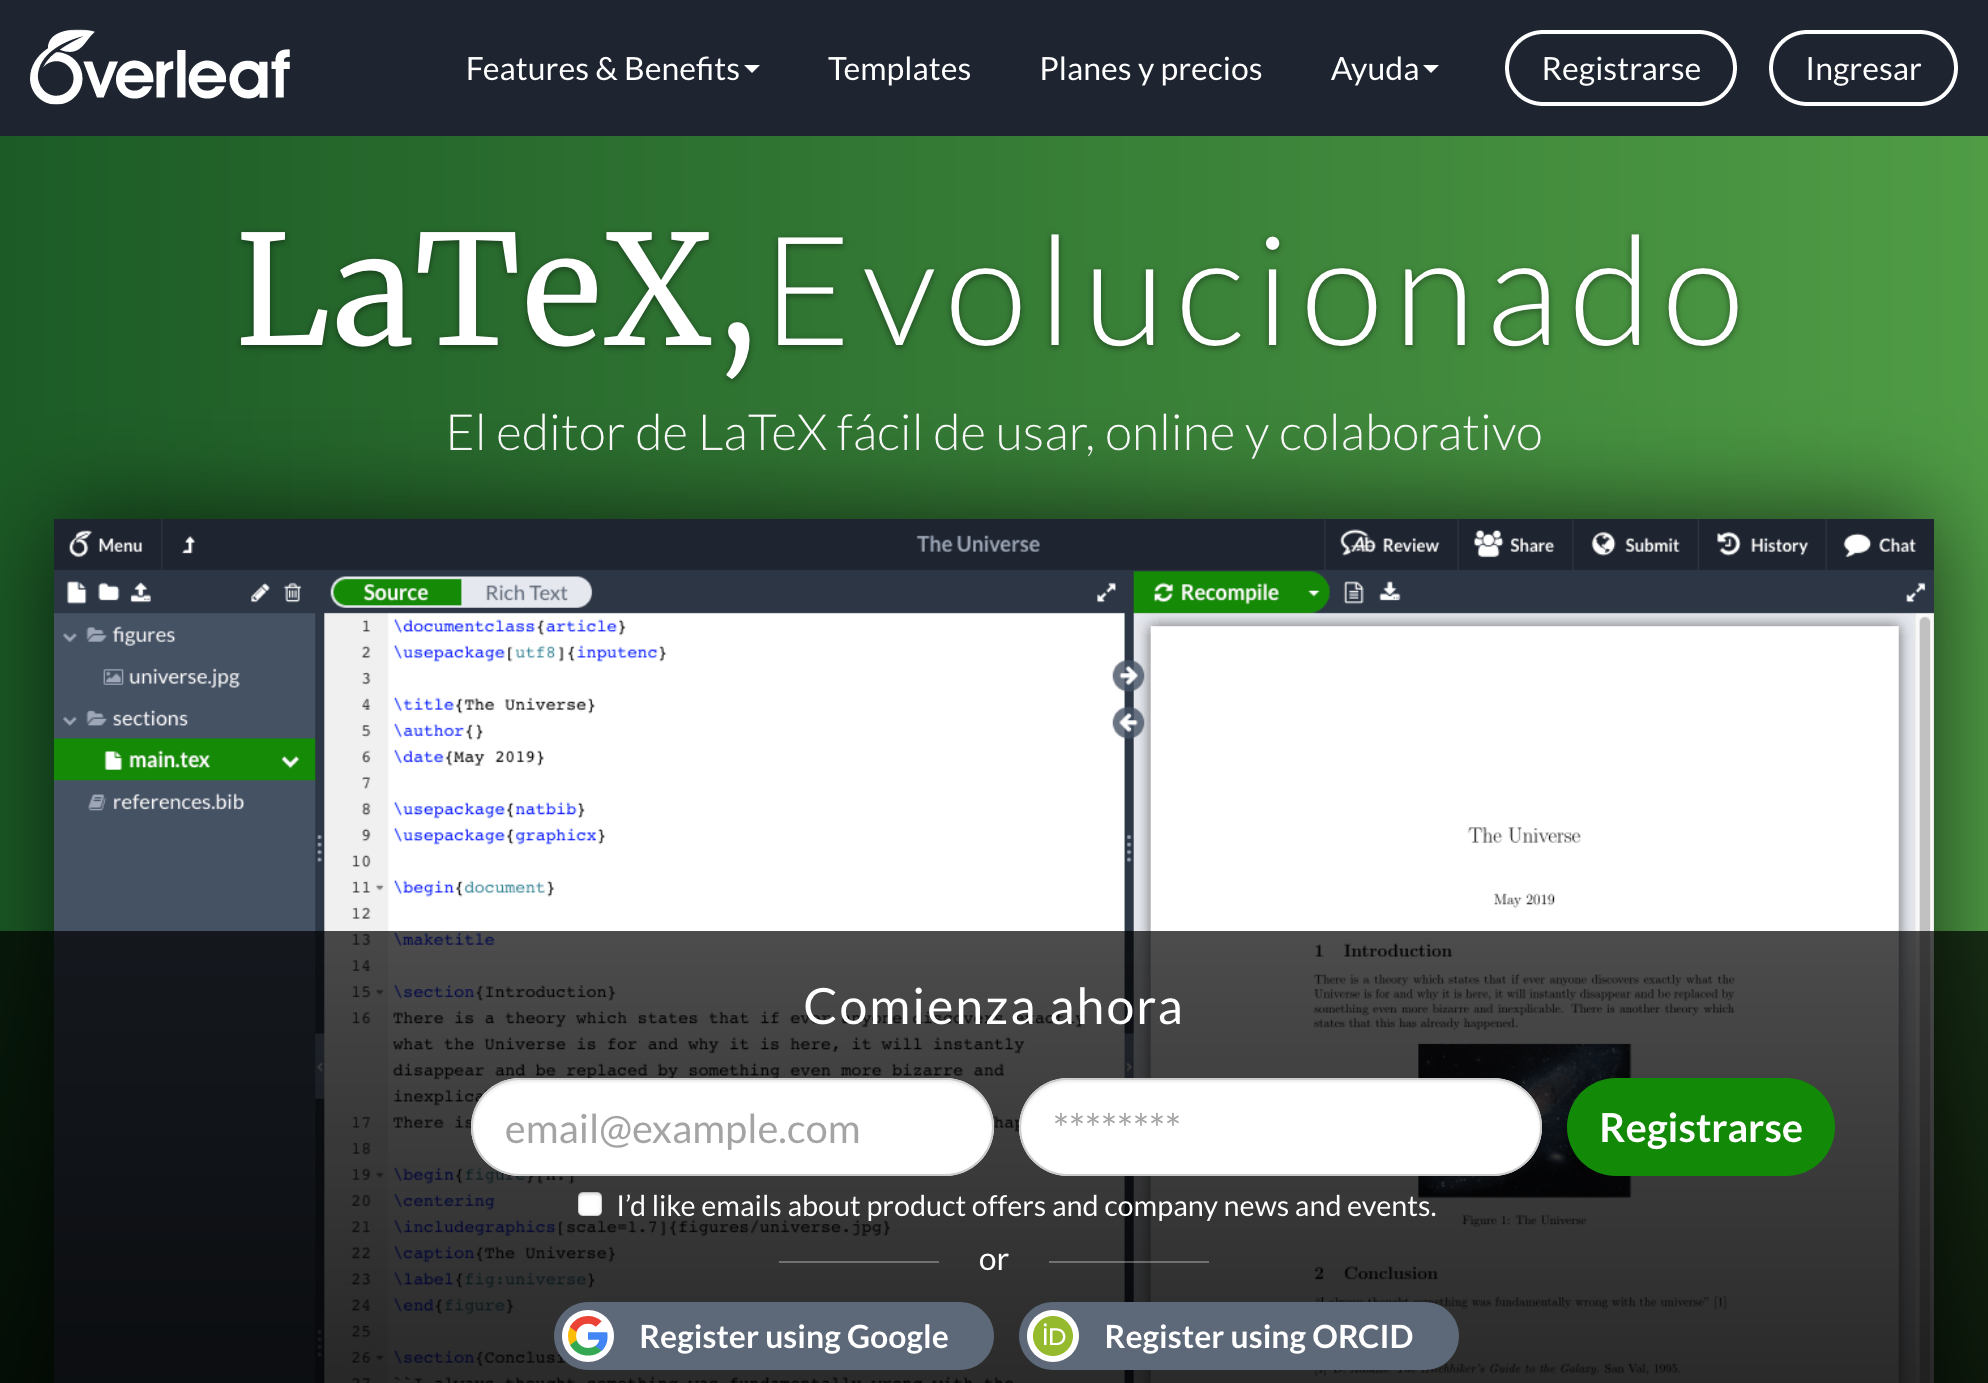
\includegraphics[width=\linewidth]{img/overleaf_300ppi.png}
	\caption{Página principal de Overleaf.}
	\label{fig:overleaf_home}
\end{figure}

En la figura \ref{fig:overleaf_home} se muestra el formulario de registro, el cual solo pide correo electrónico y contraseña, aunque también te puedes registrar mediante tu cuenta de Google. Una vez estés registrado, podemos empezar a crear el documento de prueba.



\section{Un primer documento}
\label{sec:un_primer_documento}



Dado que un documento de \LaTeX{} puede estar compuesto por muchos archivos, como después veremos, lo primero que hay que hacer es crear un proyecto (alias sofisticado de ``directorio'') en Overleaf, con \opcionMenu{Nuevo proyecto $\rightarrow$ Proyecto vacío}, como muestra la figura \ref{fig:overleaf_nuevo_proyecto_300ppi}. Aunque podemos crear proyectos a partir de ejemplos o de plantillas, empezaremos desde cero.

\begin{figure}[ht!]
	\centering
	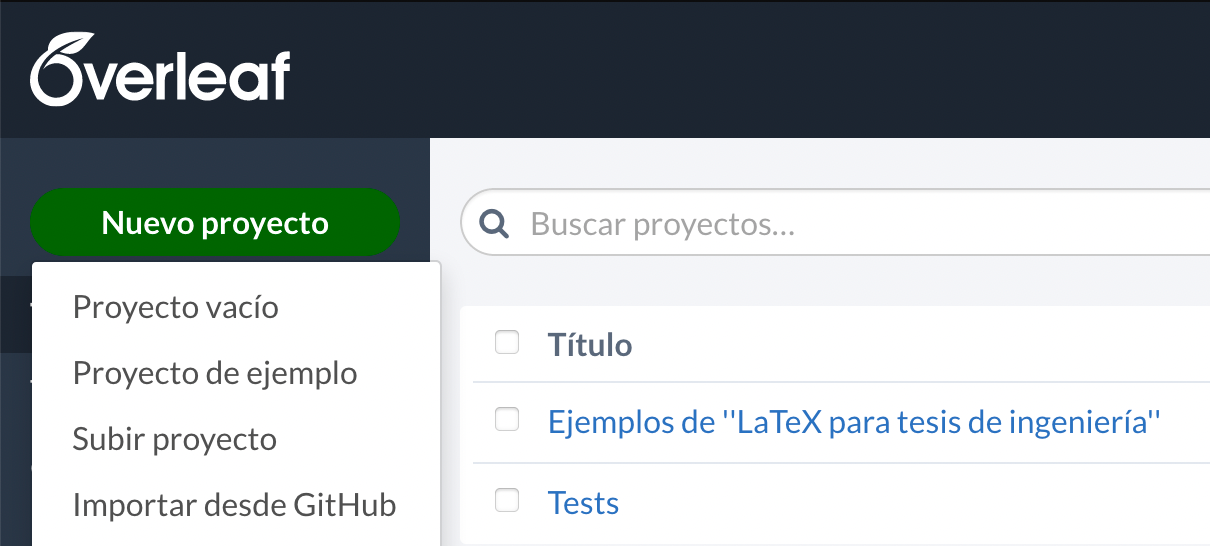
\includegraphics[scale=1]{img/overleaf_nuevo_proyecto_300ppi.png}
	\caption{Creando un nuevo proyecto en Overleaf.}
	\label{fig:overleaf_nuevo_proyecto_300ppi}
\end{figure}

Al dar clic en la opción \opcionMenu{Proyecto vacío} surgirá una pantalla modal, como la figura \ref{fig:overleaf_nombre_proyecto}, que preguntará por el nombre del proyecto. En mi caso, colocaré el nombre de \emph{Ejemplos de \textquotedbl{}LaTeX para tesis de ingeniería\textquotedbl{}}.

\begin{figure}[ht!]
	\centering
	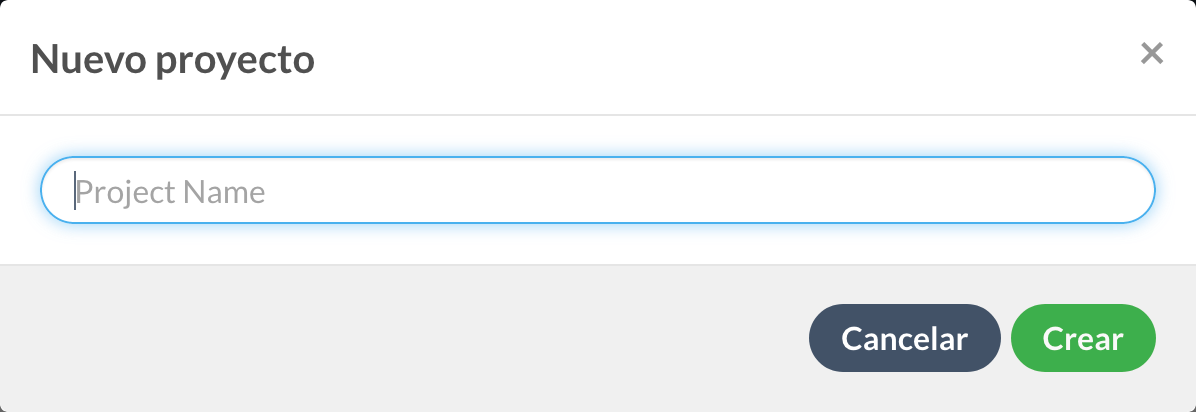
\includegraphics[width=112mm]{img/overleaf_nombre_proyecto_300ppi.png}
	\caption{Overleaf preguntando el nombre del nuevo proyecto.}
	\label{fig:overleaf_nombre_proyecto}
\end{figure}

Si todo sale bien, se desplegará una pantalla con información similar a lo que se muestra en la figura \ref{fig:overleaf_mi_primer_documento}, solo con un tamaño de fuente más pequeño. Obviamente el nombre del proyecto para ti será diferente (espero), así como el autor asignado de manera predeterminada. No obstante, en la columna izquierda debes tener un archivo llamado \texttt{main.tex}, en la columna central el contenido de dicho archivo, mientras que el lado derecho muestra el resultado en PDF con el nombre de tu proyecto, tu nombre como autor, y la fecha.

\begin{figure}[ht!]
	\centering
	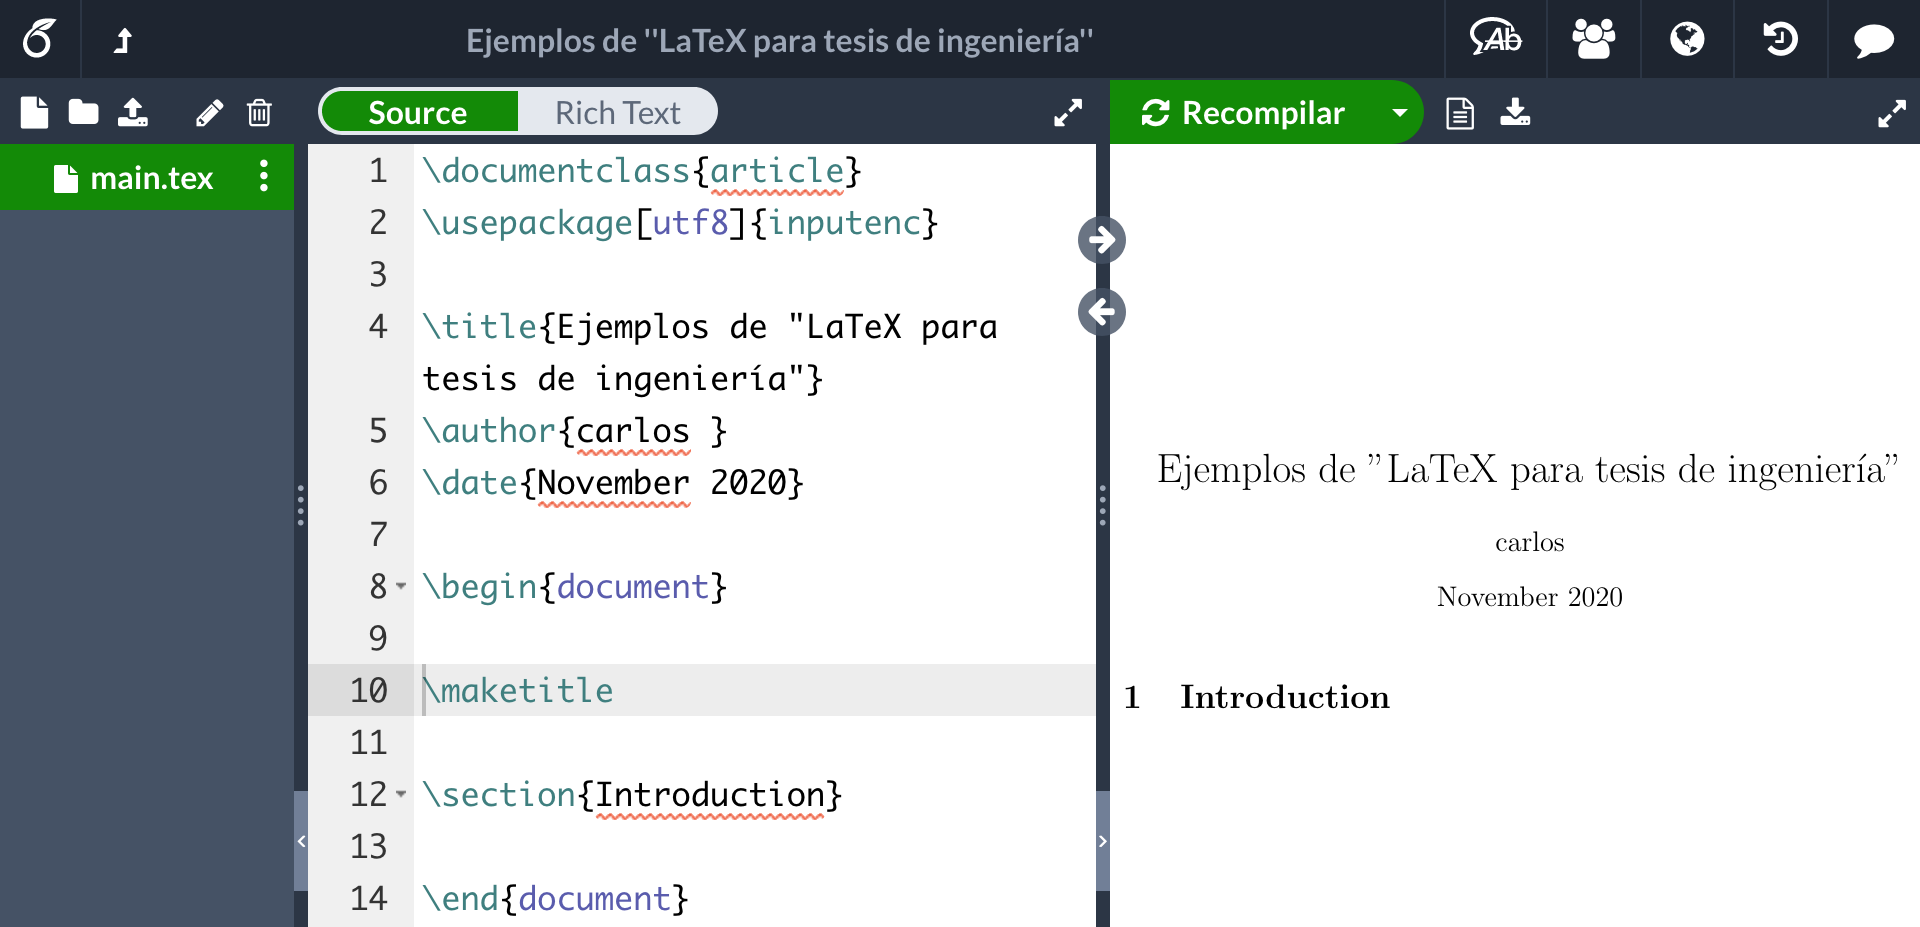
\includegraphics[width=\linewidth]{img/overleaf_mi_primer_documento_300ppi.png}
	\caption{Primer ejemplo en Overleaf.}
	\label{fig:overleaf_mi_primer_documento}
\end{figure}

Para empezar a comprender cómo funciona \LaTeX, revisemos el código del listado \ref{lst:mi_primer_documento}. En sí, lo que se puede deducir del PDF generado (lado derecho de la figura \ref{fig:overleaf_mi_primer_documento}) es que las líneas 4, 5, y 6 tienen un reflejo directo en el resultado final: se muestra el título del documento, el autor, y la fecha. También la línea 12 aparece en el documento, aunque el texto ``Introduction'' está precedido por un número.

¿Cómo es que esas cuatro líneas aparecen, una tras otra, pero en el código son separadas por la línea 8 y 10? ¿Y de dónde sale ese número asignado al texto en negritas de ``Introduction''? Y, claro, ¿por qué aparecen las comillas de cierre tanto al inicio como al final en nuestro título?

\lstinputlisting[label=lst:mi_primer_documento,numbers=left,style=latex,caption=Mi primer documento en \LaTeX.]{ejemplos/mi_primer_documento.tex}



\subsection{La instrucción \ttlatex{maketitle}}
\label{sub:la_instruccion_maketitle}



Empezaremos a responder las preguntas de manera empírica, eliminando la línea 10 del listado \ref{lst:mi_primer_documento}, que corresponde a la instrucción |\maketitle|. Se presiona el botón de \opcionMenu{Recompilar} y se observa el nuevo resultado, tal como muestra la figura \ref{fig:overleaf_sin_maketitle}.

\begin{figure}[ht!]
	\centering
	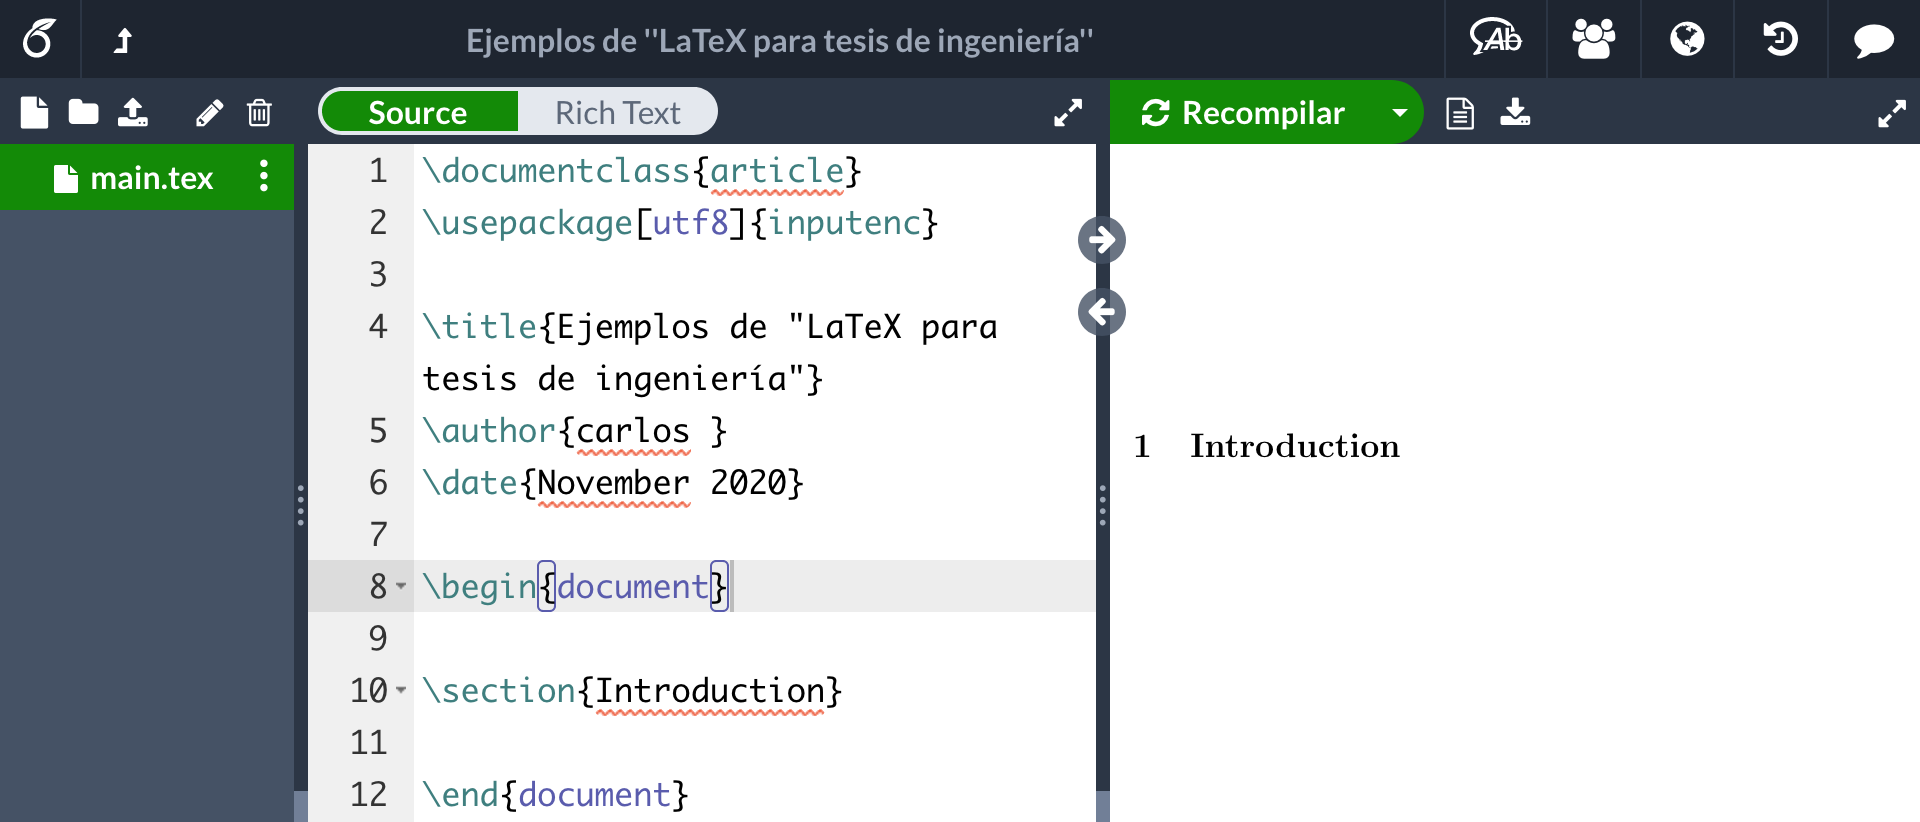
\includegraphics[width=\linewidth]{img/overleaf_sin_maketitle_300ppi.png}
	\caption{Primer ejemplo en Overleaf, sin \texttt{\textbackslash{}maketitle}.}
	\label{fig:overleaf_sin_maketitle}
\end{figure}

Dado que al eliminar la instrucción |\maketitle| ya no podemos ver en el PDF ni el título, ni el autor, ni la fecha, podemos asumir que esa instrucción se encargaba de mostrar esos tres datos centrados en el documento.

Y, basados en la misma información, podemos deducir que las instrucciones |\title|, |\author|, y |\date| son instrucciones para almacenar valores (ya que no imprimen en el documento), algo así como variables de \LaTeX, que la instrucción |\maketitle| puede leer e imprimir.

¿Importa cómo? No, solamente que lo hace. Debemos recordar que no tenemos motivos para preocuparnos por el formato o funcionalidad mientras se presente la información correcta en el documento.

Ya que sabemos los efectos de eliminar |\maketitle|, regresamos la línea a donde pertenece antes de continuar.



\subsection{La instrucción \texttt{\textbackslash{}section}}
\label{sub:la_instruccion_section}



La línea 12, |\section{Introduction}|, imprime ``Introduction'' precedido por un uno. Por ello, podemos asumir que \LaTeX, de alguna manera, enumerará consecutivamente las secciones. Haremos dos cosas para probar esta teoría:
\begin{enumerate}
	\item Cambiar el texto de ``Introduction'' a ``Introducción''.
	\item Crear una nueva sección llamada ``Esta sección debería llevar el número dos...''
\end{enumerate}

\begin{figure}[ht!]
	\centering
	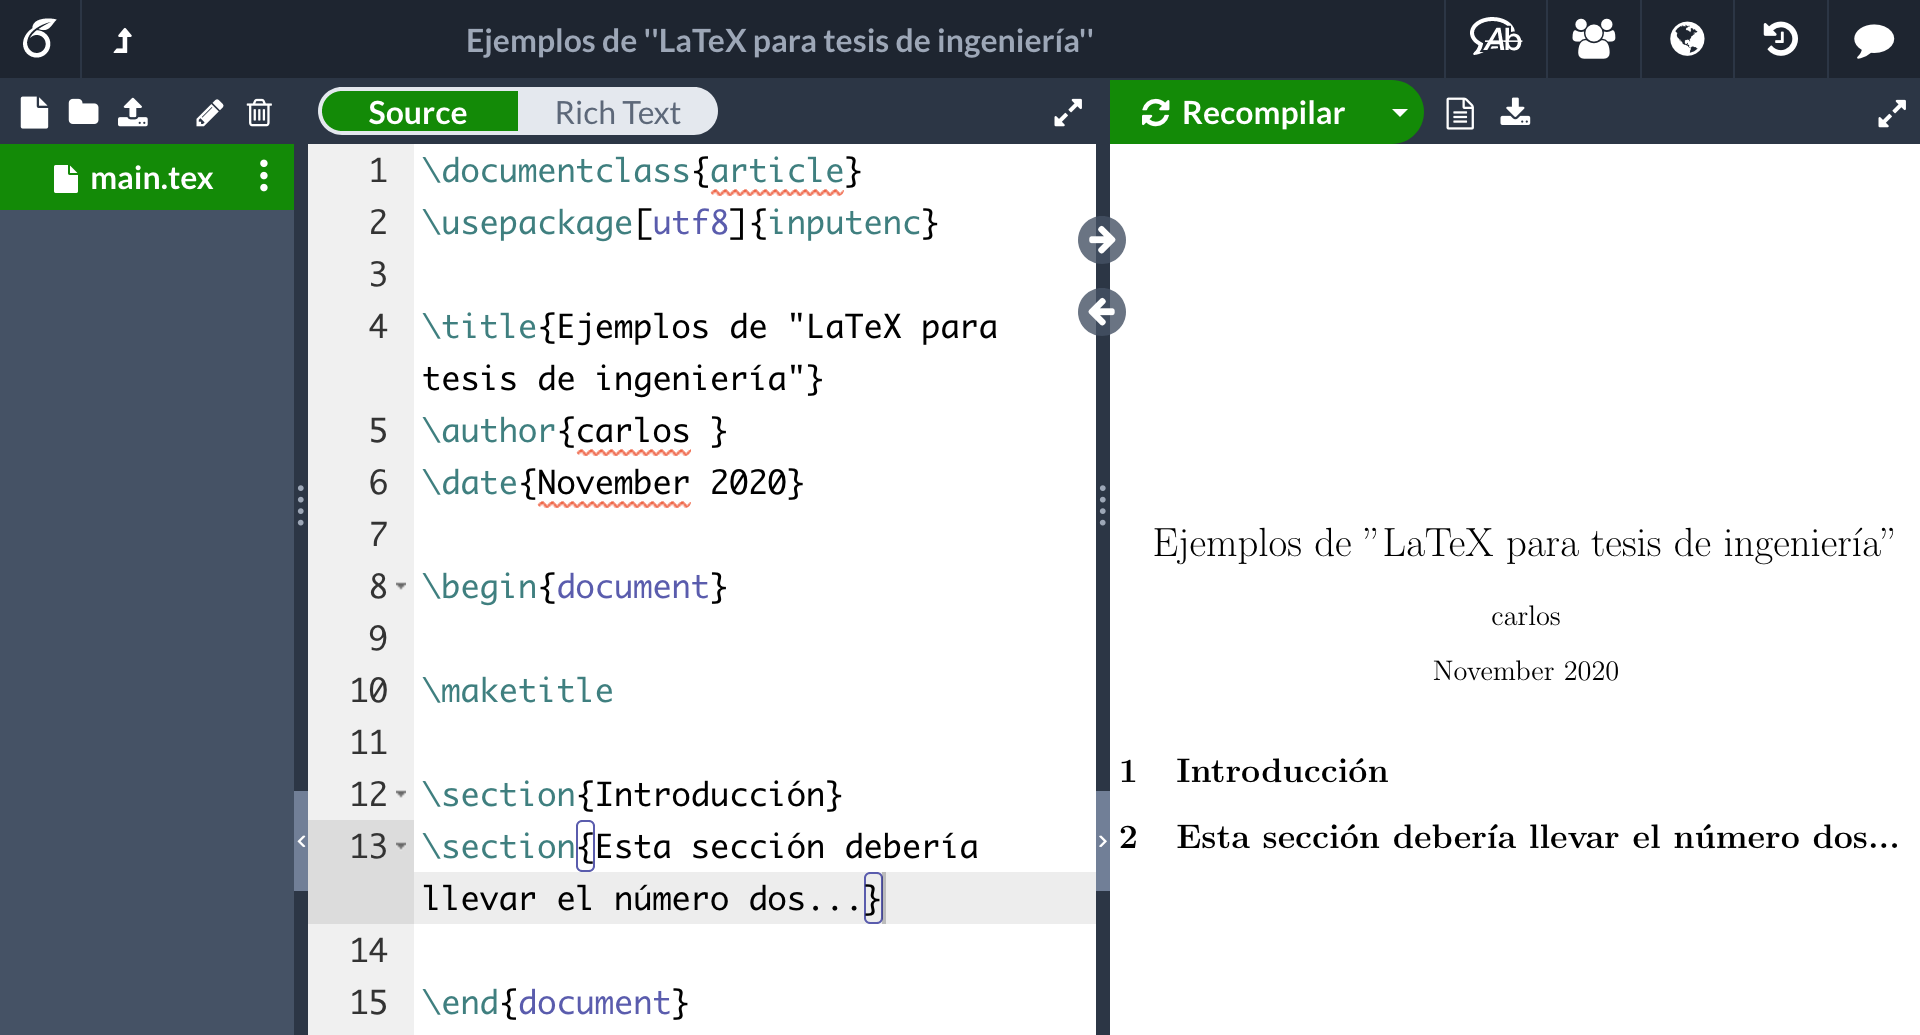
\includegraphics[width=\linewidth]{img/overleaf_seccion_dos_300ppi.png}
	\caption{Primer ejemplo en Overleaf, con una sección nueva.}
	\label{fig:overleaf_seccion_dos}
\end{figure}

La figura \ref{fig:overleaf_seccion_dos} refleja los cambios (tras volver a presionar el botón \opcionMenu{Recompilar}), y confirma las sospechas: \LaTeX{} agregará un consecutivo a cada sección, de manera automática, sin nuestra intervención (de nuevo, así nos preocupamos por la estructura del documento, no del cómo se ve). La líneas de código editadas fueron:

\begin{lstlisting}[style=latex]
\section{Introducción}
\section{Esta sección debería llevar el número dos...}
\end{lstlisting}



\subsection{Inicio y final de documento}
\label{sub:inicio_y_final_de_documento}



Siguiendo con el listado \ref{lst:mi_primer_documento}, las líneas 8 y 14 marcan el inicio y final del documento. ¿Esto qué quiere decir? Que todo lo que \emph{se ve} en el documento va entre estas dos instrucciones, por lo que si intentamos ejecutar el |\maketitle| antes de estas instrucciones, posiblemente se genere un error (y sí, la figura \ref{fig:overleaf_error_fuera_de_document} muestra el error que ocurre tras \opcionMenu{Recompilar}).

\begin{figure}[ht!]
	\centering
	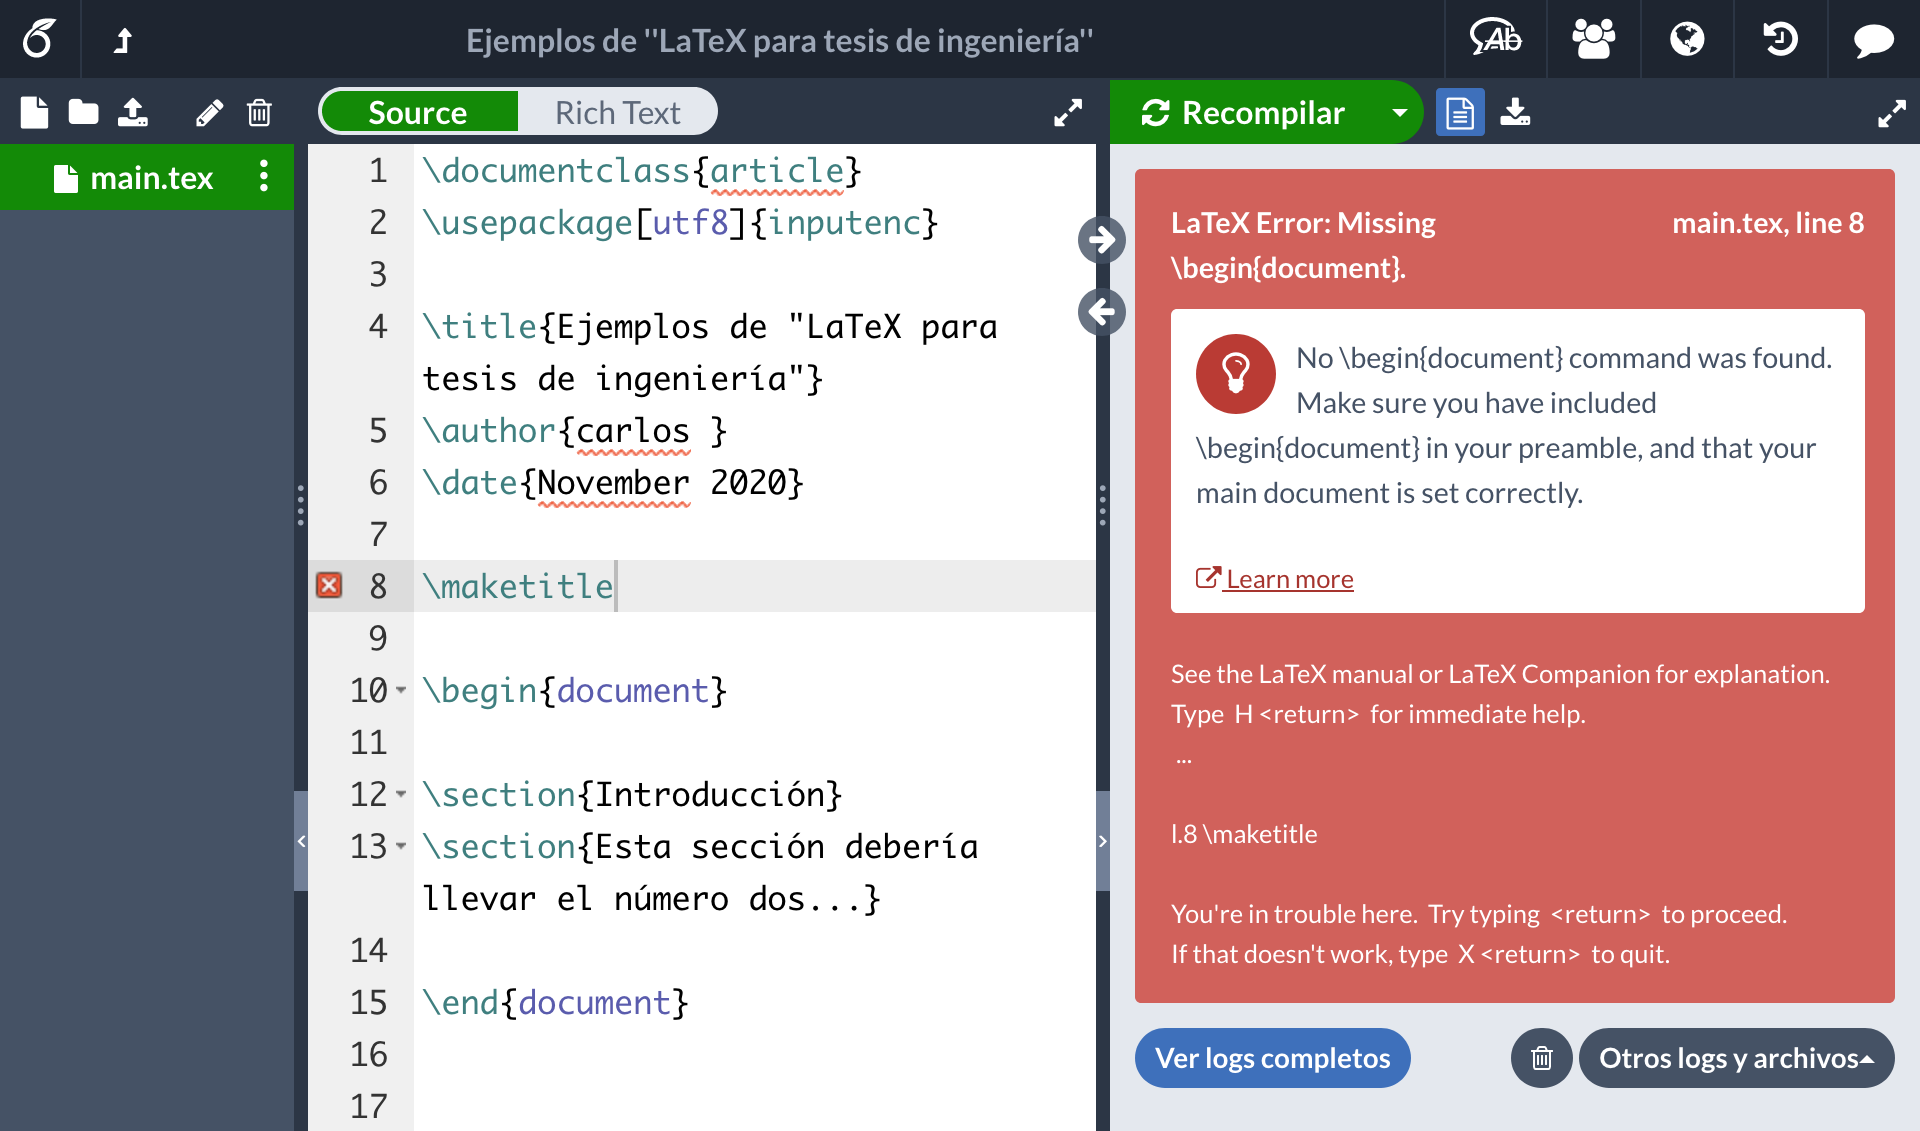
\includegraphics[width=\linewidth]{img/overleaf_error_fuera_de_document_300ppi.png}
	\caption{Primer ejemplo en Overleaf, con error fuera del \texttt{\textbackslash{}begin\{document\}}.}
	\label{fig:overleaf_error_fuera_de_document}
\end{figure}

De nuevo, no es nuestra intención conocer el cómo \LaTeX{} hace lo que hace, pero si algo va destinado a imprimirse o verse en pantalla, va entre |\begin{document}| y |\end{document}|. ¿Qué es lo que va fuera? Como en nuestro ejemplo, la declaración de ``variables'' como el autor, el título, y la fecha. También, la inclusión de paquetes que extienden las capacidades de \LaTeX{}.

En este primer documento ya se incluye el paquete \texttt{inputenc}.



\subsection{Texto en español (el paquete \texttt{\textbackslash{}inputenc})}
\label{sub:texto_en_espanol}



La instrucción |\usepackage| permite usar los paquetes que otra persona creó. Es decir, permite usar las instrucciones que alguien más ya hizo y decidió hacer públicas. Pero, en un ejemplo tan sencillo, ¿para qué necesitamos un cargar un paquete?

Cuando Donald Knuth creó \TeX{}, lo más probable es que pensara en sí mismo, sus fines, y su idioma (el inglés). Naturalmente, los acentos y las ``ñ'' no le pasaban por la mente, por lo que no son soportados de manera nativa. Para poder insertar los caracteres propios del idioma español, sin que estos sean convertidos a símbolos raros, se agrega el paquete \texttt{inputenc}, que permite definir en qué idioma estamos escribiendo (lo formal es decir algo como ``define la codificación de los caracteres de entrada'', pero se entiende menos).

Y una codificación\footnote{En inglés, \emph{encoding}.} muy utilizada, y que contiene los caracteres del español, es la UTF-8. No entraremos en detalles técnicos de representación, solo diremos que sin el paquete \texttt{inputenc} con la codificación \texttt{utf8} no se ven los caracteres en español de manera adecuada.

Como dato meramente informativo: este paquete no se incluye solamente porque tu Overleaf se haya configurado en español. El código ASCII quedó atrás hace mucho tiempo, siendo el UTF-8 el nuevo estándar de codificación. Así que, aunque tu documento solo utilice caracteres del idioma inglés, se recomienda utilizar el paquete UTF-8 (razón por la que Overleaf lo carga de manera predeterminada).



\subsection{Clase del documento}
\label{sub:clase_del_documento}



Dejamos la primera línea para el final, donde se define la clase del documento. Hay varias clases de documento, y muchas más si contamos las plantillas como el \href{https://www.latextemplates.com/template/tufte-style-book}{libro Tufte}, pero a lo largo de este libro utilizaremos artículos (clase \texttt{article}) y libros (clase \texttt{book}).

Los artículos serán utilizados para hacer las demostraciones cortas, como el listado \ref{lst:mi_primer_documento}, y el libro es la base de este documento, del cual tienes todo el código fuente a tu disposición.

Aunque existen muchas diferencias entre ambas clases, una de las principales es la estructura, o la forma en la que se subdivide, como se muestra en las siguientes listas:

\begin{multicols}{2}
Libro
\begin{itemize}
	\item Capítulo
	\begin{itemize}
		\item Sección
		\begin{itemize}
			\item Subsección
		\end{itemize}
	\end{itemize}
\end{itemize}

\columnbreak

Artículo
\begin{itemize}
	\item Sección
	\begin{itemize}
		\item Subsección
	\end{itemize}
\end{itemize}
~
\end{multicols}

Dicho de otra forma, un libro tiene más subdivisiones porque cuenta con separación por capítulos mientras que un artículo define su nivel principal a través de secciones.

La otra diferencia es que un artículo coloca el título en la primera hoja, seguido de todo el contenido (lo cual vimos en las figuras \ref{fig:overleaf_sin_maketitle} y \ref{fig:overleaf_seccion_dos}), mientras que un libro crea una portada y comienza el contenido principal a partir de la segunda hoja (como en este mismo documento).

Al experimentar con la clase \texttt{book} solo ten en cuenta que si no tienes un capítulo (|\chapter|), las secciones estarán numeradas como ``0.1'' y ``0.2'', por la falta del nivel superior.



\section{¿Compilar, recompilar?}
\label{sec:_compilar_recompilar_}



Al momento de regenerar el documento dimos clic al botón \emph{Recompilar}, el cual hace la magia que actualiza el documento PDF. Pero ¿qué es? ¿qué hace? ¿por qué tenemos que presionarlo para ver cada cambio?

Dentro de las características de \LaTeX{} se mencionó que no era un editor \emph{WYSIWYG}, lo que implica que al escribir no veremos lo recién escrito en la forma que aparecerá en el documento PDF. Y, si recuerdas la figura \ref{fig:esquema_latex}, hablamos de intrucciones que nos ayudaban a enfocarnos en el contenido, y que esas instrucciones luego se convertían en el documento con formato.

Pero, ¿cómo es que esas instrucciones pasan de lo que escribimos al documento final? El verbo que buscamos es \emph{compilar}. Aquí lo definiremos como:

\begin{displayquote}
La traducción de las instrucciones \textbf{válidas} de \LaTeX{} a un documento hermoso, digno de ser mostrado como tesis.
\end{displayquote}

Es importante el énfasis en la palabra ``válidas''. En Word, si haces algo que no le gusta, desacomoda todo el documento, cosa que arreglas con un \opcionMenu{Ctl + Z}. En \LaTeX{}, si haces algo que no le gusta, no tendrás documento de salida. Nada, cero, inexistente... como tu calificación (tú no te preocupes, para eso tienes este libro).

Siguiendo con el vocabulario: si ya compilaste una vez, la siguiente vez será una \emph{recompilación} (por eso Overleaf utiliza \emph{recompilar}, porque automáticamente genera el PDF la primera vez). A lo largo de este documento no se hace distinción entre ambas acciones: compilar y recompilar se usan de manera intercambiable.



\subsection{Compila frecuentemente}
\label{ssec:compila_frecuentemente}



Antes de continuar, aventurero, escucha mi advertencia: recuerda compilar frecuentemente. ¡Compila, compila! ¿Escribes una línea? Compila. ¿Escribes un párrafo? Compila. ¿Agregas una nueva imagen? Compila. ¿Cambiaste un acentito? Compila.

Créeme, cualquier cosa insospechada puede causar error. Luego, cuando tengas todo un capítulo escrito pero no puedas ver nada mas que errores sobre errores, odiarás \LaTeX{}. Solo confía en mí: compila con la misma paranoia con la que guardas el documento.



\section{Archivos temporales}
\label{sec:archivos_temporales}



En esta obra no veremos cómo es que \LaTeX{} hace su magia (bueno, un poco, y hasta el final), pero hay que responder a la pregunta: ¿dónde pone \LaTeX{} todo lo que necesita para pasar de nuestro texto plano al PDF final?

Después de todo, requiere mantener un contador de en qué capítulo y en qué sección va, traducir comandos a texto dispuesto en el PDF, obtener los valores de variables como el autor o la fecha, entre otras fechorías más.

Debido a todo lo que tiene que hacer, el proceso de compilación genera archivos temporales para ayudarle a llegar del texto plano al documento final. Algunas de las extensiones de los archivos generados en el proceso son: \texttt{*.toc}, \texttt{*.lof}, \texttt{*.bbl}, \texttt{*.aux}, entre otras.

No ocupamos saber para qué requiere tanto archivo, mientras haga bien su trabajo... y es ahí donde viene un problema. Cuando nosotros cometemos un error, e indefectiblemente lo haremos, el compilador no puede acabar su tarea. ¿Y eso qué? Volvemos a iniciar el proceso de compilación y ya, ¿no?

Sí... y no. Como al compilador le gusta ser eficiente, si unos archivos no han presentado cambios entonces no los reescribe con el fin de ahorrar tiempo, lo que puede terminar con un error que se ha quedado guardado en un archivo temporal.

Dicho de otro modo, podemos tener errores fantasma que ya fueron solucionados en el código fuente pero que se han quedado atorados en los archivos temporales. Y es por esta razón que es necesario hablar de ellos: debes saber cómo eliminarlos para cuando tengas un error persistente, para descartar la posibilidad de que el error solo exista en un archivo temporal.

Overleaf nos da la opción de eliminar los archivos temporales, aunque no hay un botón de tan fácil acceso como \opcionMenu{Recompilar}. Para eliminar los archivos primero tenemos que ubicar el botón de \opcionMenu{Logs y archivos de salida}, que se encuentra justo al lado derecho del botón \opcionMenu{Recompilar}, como que se muestra en la figura \ref{fig:overleaf_boton_log}.

\begin{figure}[ht!]
	\centering
	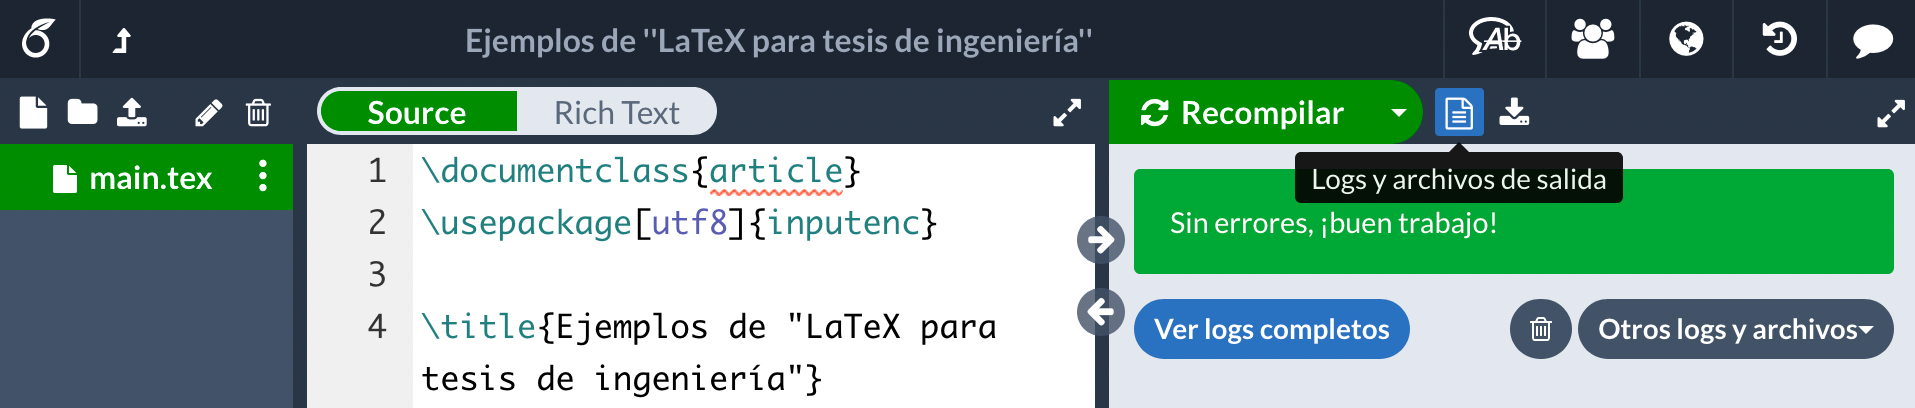
\includegraphics[width=\linewidth]{img/overleaf_boton_log_300ppi.png}
	\caption{Botón de \opcionMenu{Logs y archivos de salida} en Overleaf.}
	\label{fig:overleaf_boton_log}
\end{figure}

Al dar clic sobre dicho botón se abrirá un pequeño menú, como se muestra en la figura \ref{fig:overleaf_boton_cache}, que nos da acceso al botón \opcionMenu{Borrar archivos en la caché}, con el ícono de un bote de basura, que nos permite deshacernos de los archivos temporales asociados al proceso de compilación de nuestro proyecto o archivo.

\begin{figure}[ht!]
	\centering
	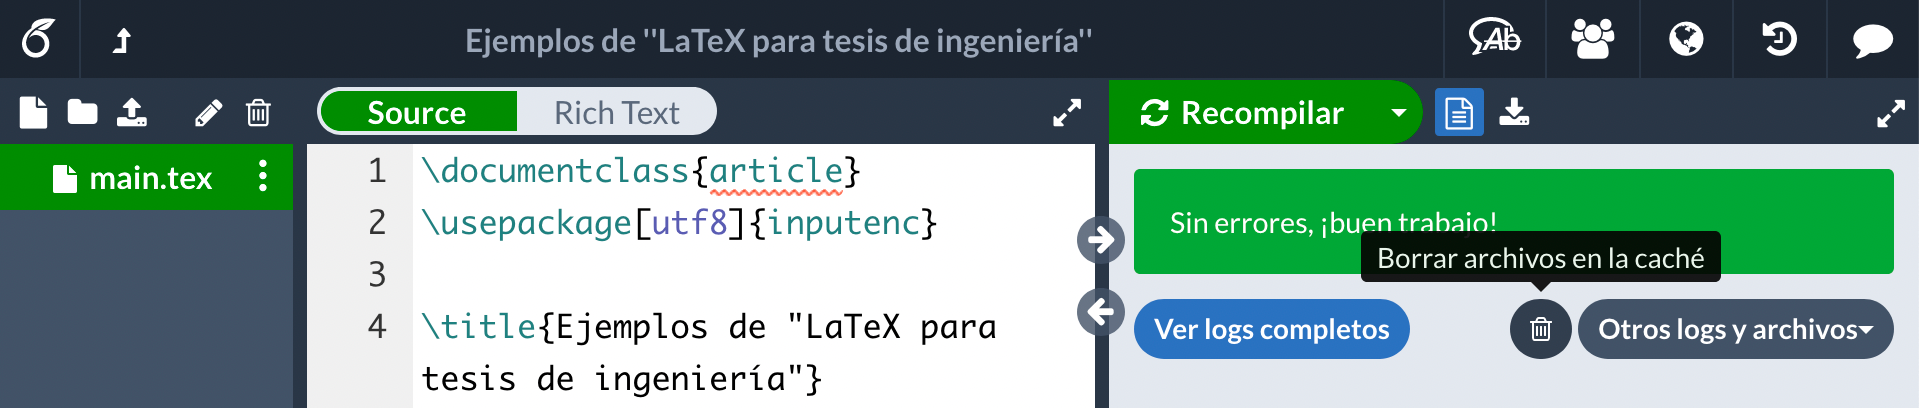
\includegraphics[width=\linewidth]{img/overleaf_boton_cache_300ppi.png}
	\caption{Botón de \opcionMenu{Borrar archivos en la caché} en Overleaf.}
	\label{fig:overleaf_boton_cache}
\end{figure}



\newpage
\section*{Resumen}



En este capítulo definimos qué es \LaTeX{} de una manera que facilita su interacción con el sistema e indagamos empíricamente qué hace cada línea del primer documento generado en la plataforma en línea Overleaf.

Además, establecimos dos consejos que te ayudarán mucho en tu aventura de terminar tu tesis con \LaTeX{}: compila frecuentemente y elimina archivos temporales después de una compilación fallida.

Armados con este conocimiento, estamos listos para empezar a ver cómo usar negritas, cursivas, y otras cosas de formato en \LaTeX{}.
% \input{Más capítulos...}

\end{document}
\end{lstlisting}



\section{Márgenes del documento}
\label{sec:margenes}



Para cambiar los márgenes del documento requerimos de otro paquete:

\begin{lstlisting}[style=latex]
\usepackage{geometry}
\end{lstlisting}

Aunque al incluir los paquetes se pueden establecer los nuevos márgenes, mi preferencia es realizar la configuración con una instrucción aparte, que se incluirá en el archivo \texttt{package-conf.tex} (porque debe estar después de incluir el paquete pero antes del |\begin{document}|).

La instrucción a utilizar es |\geometry|, la cual tiene muchas opciones de configuración (las cuales se pueden ver en \cite{bib:geometry_package}). Las opciones que necesitamos para configurar los márgenes son cuatro:
\begin{enumerate}
	\item \texttt{tmargin}, para el margen superior (del inglés \emph{top margin}).
	\item \texttt{bmargin}, para el margen inferior (del inglés \emph{bottom margin}).
	\item \texttt{rmargin}, para el margen derecho (del inglés \emph{right margin}).
	\item \texttt{lmargin}, para el margen izquierdo (del inglés \emph{left margin}).
\end{enumerate}

Y esto aplica específicamente para este libro digital, cuyo objetivo no es ser impreso. En caso de ser así, tendría que considerar que las páginas se imprimen por ambos lados, y que el documento tendrá un lomo, por lo que el margen interno (cercano al lomo) es diferente al margen externo (la parte de la hoja que tomamos para dar la vuelta a la página). Para expresar eso tenemos las opciones de \texttt{inner} para margen interno, y \texttt{outer} para margen externo. La opción de \texttt{twoside} permite establecer que los parámetros que se prefieren son \texttt{inner} y \texttt{outer} sobre \texttt{left} y \texttt{right}.

No obstante, ¿los márgenes se dan respecto a qué tamaño de hoja? De manera predeterminada, \LaTeX{} utiliza el tamaño de papel A4, aunque muchos más se pueden utilizar. Por ejemplo, está la opción \texttt{letterpaper}, \texttt{legalpaper}, \texttt{a0paper}, \texttt{a1paper}, \texttt{b4paper}, y más (la lista completa está en la sección 5.1 de \cite{bib:geometry_package}). Incluso se puede definir un tamaño personalizado, con las opciones \texttt{paperwidth} y \texttt{paperheight}.

Para una tesis se recomienda el tamaño carta, y ya dependerá de los requisitos si es impresión por un lado o por dos. Como ejemplo, se establece el tipo de papel como tamaño carta, con márgenes inferior y superior de 2cm, y márgenes laterales de 3cm, con la instrucción:

\begin{lstlisting}[style=latex]
\geometry{
	verbose,letterpaper,     % Tamaño carta, con mensajes de advertencia.
	tmargin=2cm,bmargin=2cm, % Margen superior e inferior.
	lmargin=3cm,rmargin=3cm  % Margen izquierdo y derecho.
}
\end{lstlisting}

La opción \texttt{verbose} indica que se debe mostrar una advertencia en terminal cuando algo en el texto salga de los márgenes establecidos. En sí, es un opción que ayuda al momento de estar redactando y compilando el documento, para captar más rápido algunos problemas de visualización antes de verlos realmente en el PDF.



\section{Colores}
\label{sec:colores}



No todo en \LaTeX{} es texto de color negro, podemos incluir colores, \textcolor{red}{como en este pedazo de línea}, o \textcolor{blue}{este otro}. En código, el texto anterior luce como:

\begin{lstlisting}[style=latex]
\textcolor{red}{como en este pedazo de línea}, % texto en color rojo.
o \textcolor{blue}{este otro}.                 % texto en color azul.
\end{lstlisting}

Es decir, la instrucción |\textcolor| recibe dos parámetros necesarios: primero el color, después el texto que sufrirá el cambio.

Pero, ¿qué colores están definidos? ¿será acaso que la instrucción |\textcolor| y los colores están definidos sin tener que agregar otro paquete? ¡Por favor! Espero que no hayas hecho esa pregunta, obviamente pertenece a otro paquete: \texttt{xcolor}. Respecto a la primera pregunta, la documentación en \cite{bib:xcolor_package} muestra la lista de colores base siempre disponibles en su sección 4, replicada aquí debajo:

\begin{multicols}{5}
\noindent\fcolorbox{black}{black}{\rule{0pt}{4pt}\rule{4pt}{0pt}}~\emph{black}\\
\fcolorbox{black}{blue}{\rule{0pt}{4pt}\rule{4pt}{0pt}}~\emph{blue}\\
\fcolorbox{black}{brown}{\rule{0pt}{4pt}\rule{4pt}{0pt}}~\emph{brown}\\
\columnbreak
\fcolorbox{black}{cyan}{\rule{0pt}{4pt}\rule{4pt}{0pt}}~\emph{cyan}\\
\fcolorbox{black}{darkgray}{\rule{0pt}{4pt}\rule{4pt}{0pt}}~\emph{darkgray}\\
\fcolorbox{black}{gray}{\rule{0pt}{4pt}\rule{4pt}{0pt}}~\emph{gray}\\
\fcolorbox{black}{green}{\rule{0pt}{4pt}\rule{4pt}{0pt}}~\emph{green}\\
\columnbreak
\fcolorbox{black}{lightgray}{\rule{0pt}{4pt}\rule{4pt}{0pt}}~\emph{lightgray}\\
\fcolorbox{black}{lime}{\rule{0pt}{4pt}\rule{4pt}{0pt}}~\emph{lime}\\
\fcolorbox{black}{magenta}{\rule{0pt}{4pt}\rule{4pt}{0pt}}~\emph{magenta}\\
\fcolorbox{black}{olive}{\rule{0pt}{4pt}\rule{4pt}{0pt}}~\emph{olive}\\
\columnbreak
\fcolorbox{black}{orange}{\rule{0pt}{4pt}\rule{4pt}{0pt}}~\emph{orange}\\
\fcolorbox{black}{pink}{\rule{0pt}{4pt}\rule{4pt}{0pt}}~\emph{pink}\\
\fcolorbox{black}{purple}{\rule{0pt}{4pt}\rule{4pt}{0pt}}~\emph{purple}\\
\fcolorbox{black}{red}{\rule{0pt}{4pt}\rule{4pt}{0pt}}~\emph{red}\\
\columnbreak
\fcolorbox{black}{teal}{\rule{0pt}{4pt}\rule{4pt}{0pt}}~\emph{teal}\\
\fcolorbox{black}{violet}{\rule{0pt}{4pt}\rule{4pt}{0pt}}~\emph{violet}\\
\fcolorbox{black}{white}{\rule{0pt}{4pt}\rule{4pt}{0pt}}~\emph{white}\\
\fcolorbox{black}{yellow}{\rule{0pt}{4pt}\rule{4pt}{0pt}}~\emph{yellow}\\
\end{multicols}

No obstante, esos colores no son suficientes. El mismo paquete define otros colores, definidos en espacios de nombres como \texttt{dvipsnames}, \texttt{svgnames}, o \texttt{x11names}. Para este documento yo elegí los colores presentes en \texttt{svgnames}, por lo tanto, esta es la manera de incluir el paquete:

\begin{lstlisting}[style=latex]
\usepackage[svgnames]{xcolor} % Colores para el código, portada, etc.
\end{lstlisting}

Por supuesto, de momento no parece algo demasiado útil, ¿por qué querríamos cambiar el color de una línea de texto así? ¿qué aplicaciones tiene? Un primer ejemplo es la portada de este documento, la cual fue hecha con \LaTeX{}. Para ello, el color de la página fue cambiado, al igual que el color del texto. Dichos cambios se realizaron con las siguientes instrucciones:

\begin{lstlisting}[style=latex]
\pagecolor{DeepPink!40!Black} % Cambia el color de fondo de la página.
\color{White}                 % Cambia el color de fonde del texto.
\end{lstlisting}

La instrucción |\pagecolor| sirve para cambiar el color de la página, y la instrucción |\color| cambia el color del texto. Ambas reciben un único parámetro obligatorio: el color.

Los colores utilizados fueron tres, \texttt{DeepPink}, \texttt{Black}, y \texttt{White}, los cuales están definidos en el espacio de nombres \texttt{svgnames} (los colores básicos son \texttt{black} y \texttt{white}, todo en minúsculas).

No obstante, el color de fondo no se define exclusivamente mediante \texttt{DeepPink}, sino que es \texttt{DeepPink!40!Black}, ¿qué significa? Para eso se tendría que entender el modelo de color de \LaTeX{}, que se explica en \cite{bib:latex_colors} y \cite{bib:xcolor_model}, pero lo básico se puede entender con la siguiente formulita:

\[
\texttt{DeepPink!40!Black} = 40\%~\texttt{DeepPink} + 60\%~\texttt{Black}
\]

Es decir, lo que hacemos en esa mezcla es oscurecer el color \texttt{DeepPink}. Si quisieramos realizar la operación contraria, de hacerlo más claro, podemos omitir el segundo color pues automáticamente se mezcla con blanco:

\[
\texttt{DeepPink!40} = 40\%~\texttt{DeepPink} + 60\%~\texttt{White}
\]

Una vez que tienes un color que te gusta, puedes asignarle un nombre. Por ejemplo, a esta mezcla la podemos llamar \texttt{FondoPortada} usando la instrucción |\colorlet|:

\begin{lstlisting}[style=latex]
\colorlet{FondoPortada}{DeepPink!40!Black}
\end{lstlisting}

Así puedes generar toda tu paleta de colores, con referencia a tus colores propios. Estas definiciones van en el preámbulo, después de agregar el paquete \texttt{xcolor}. Sí: en el archivo \texttt{package-conf.tex}. Así es como empieza a crecer.

Con esa nueva definición podemos cambiar el código de la portada para usar nuestro nuevo color:

\begin{lstlisting}[style=latex]
\pagecolor{FondoPortada} % Cambia el color de fondo de la página.
\color{White}            % Cambia el color de fonde del texto.
\end{lstlisting}

También podemos definir colores que no se basen en otro color, mediante su valor de RGB (cantidad de rojo, verde, y azul). Por ejemplo, si usamos el modelo \texttt{rgb} podemos utilizar valores de cada color entre 0 y 1, por lo que la siguiente instrucción crea un gris tenue, 96\% blanco:

\begin{lstlisting}[style=latex]
\definecolor{Resaltado}{rgb}{0.96, 0.96, 0.96}
\end{lstlisting}

En sí, podemos utilizar la instrucción |\definecolor| para definir un color desde cero, o la |\colorlet| para derivar un color nuevo en base a una mezcla de otros existentes.



\section{Enlaces}
\label{sec:enlaces}



En este documento, las referencias a figuras, tablas, código, y ecuaciones están enlazadas a aquello a lo que hacen referencia. Es decir, al dar clic sobre un numerito, este te lleva a la sección, figura, etcétera, a lo que hagan referencia.

Esta característica es algo completamente inútil en un libro impreso (obviamente, espero), pero este PDF está diseñado para ser un documento digital, y las referencias se muestran en color diferente al texto normal. Esto se hace gracias a tres cosas:
\begin{enumerate}
	\item El uso del paquete \texttt{hyperref}.
	\item La configuración de cómo se muestran los enlaces a referencias.
	\item El color diferente, que podemos definir gracias al paquete \texttt{xcolor}.
\end{enumerate}

Es decir, \LaTeX{} no provee esos enlaces de manera predeterminada, pero la inclusión del paquete \texttt{hyperref} hace toda la magia por nosotros. Con agregar la instrucción |\usepackage{hyperref}| se crean todos los enlaces a las referencias, con un solo problemita: se ven algo feas.

Sin configuración apropiada, las referencias se muestran encerradas en recuadros rojos que no son exactamente agradables a la vista, como se ve en \cite{bib:overleaf_hyperref}. Por fortuna, podemos cambiar cómo se muestran gracias a la instrucción |\hypersetup|.

En lugar de subrayar los enlaces, podemos cambiarlos de color con la opción de \texttt{colorlinks}. También, como los URLs\footnote{En español son \emph{LRU}, o ``localizador de recursos uniforme''... pero dudo que alguien los llame así.} pueden ser muy largos, activamos la opción de \texttt{breaklinks} para permitirle al compilador romper los enlaces en varias líneas, en caso de ser necesario.

Por último, establecemos el color de los enlaces a páginas web, de las citas, y de los otros elementos al mismo color, el color \texttt{Enlaces}:

\begin{lstlisting}[style=latex]
\hypersetup{
	colorlinks,        % Usamos color en lugar de caja roja.
	breaklinks,        % Permite dividir el enlace si es muy largo.
	urlcolor=Enlaces,  % Color a páginas web con \url.
	citecolor=Enlaces, % Color de referencias con \cite.
	linkcolor=Enlaces  % Color de \ref y \footnote.
}
\end{lstlisting}

Y el color \texttt{Enlaces} lo definimos en el mismo preámbulo, antes del |\hypersetup|:

\begin{lstlisting}[style=latex]
\colorlet{Enlaces}{FondoPortada}
\end{lstlisting}

Sí, el color \texttt{Enlaces} puede ser solamente un alias de otro color (en este caso, de \texttt{FondoPortada}). No obstante, si posteriormente quiero cambiar el color de los enlaces, puedo hacerlo desde el |\colorlet|, en lugar de buscar el |\hypersetup|.



\section{Texto resaltado}
\label{sec:texto_resaltado}



En caso de requerir resaltar texto en tu documento puedes utilizar la instrucción |\hl| (reducción de \emph{highlight}), que viene incluida con el paquete \hl{\texttt{soul}}. Para resaltar la palabra \hl{\texttt{soul}} se utilizó el código |\hl{\texttt{soul}}|. El discreto color amarillo es el valor predeterminado del resaltado, cual si fuera marcatextos.

No obstante, para el idioma español se requiere el paquete \texttt{soulutf8} para que la instrucción |\hl| acepte acentos. En sí, \texttt{soulutf8} es un parche sobre el paquete \texttt{soul} que añade algo de compatibilidad con UTF-8 (así lo dice la misma documentación oficial del paquete en \cite{bib:soulutf8_package}). Solo usa \texttt{soulutf8} en lugar de \texttt{soul} solamente.

El comando \instruccionlatex{hl\{texto\}} solo funciona si un paquete de color ha sido cargado (como el \texttt{xcolor}). Si el amarillo chillante no parece demasiado útil, se puede cambiar a un color más discreto en cualquier parte del documento, incluyendo el preámbulo para hacer el cambio global. Aquí podemos cambiar al gris claro definido previamente:

\sethlcolor{Resaltado}
\begin{lstlisting}[style=latex]
\sethlcolor{Resaltado}
\end{lstlisting}

Esto nos permite usar un fondo sutil para resaltar código, como la instrucción \hl{\texttt{\textbackslash{}hl}} o \hl{\texttt{\textbackslash{}usepackage}}. Aunque si lo discreto no es lo nuestro, podemos elegir el color \texttt{DeepPink} para cambiar de color otra vez:
\begin{lstlisting}[style=latex]
\sethlcolor{DeepPink}
\end{lstlisting}

\sethlcolor{DeepPink}
\noindent y luego proceder a \hl{resaltar este texto con color rosa}. También podemos alterar un solo resaltado encerrando el contenido entre llaves junto con el cambio de color, |{\sethlcolor{green} \hl{texto resaltado en verde}}|, lo que resulta en {\sethlcolor{green} \hl{texto resaltado en verde}} que no afecta al siguiente \hl{resaltado}.

\sethlcolor{Resaltado}
\noindent Podemos resumir el uso del resaltado con las siguientes instrucciones:
\begin{lstlisting}[style=latex]
\usepackage{soulutf8} % Colocar en el preámbulo para poder resaltar.

\sethlcolor{Resaltado} % Cambia el color de resaltado de aquí en delante.
{\sethlcolor{Resaltado} cambio de una vez}  % Cambia el color solo aquí.
\hl{texto} % Instrucción para resaltar texto.
\end{lstlisting}



\section{Definición de instrucciones}
\label{sec:Definicion_de_instrucciones}



Supongamos ahora que se quiere establecer como estándar que el texto de ancho fijo aparezca resaltado por un leve tono de gris. Eso implica el uso de dos instrucciones en serie: |\texttt{\hl{texto en ancho fijo resaltado}}|. Dos instrucciones, dos pares de llaves a cerrar.

Con el fin de evitar errores con las llaves, podemos unificar los dos comandos en uno mediante la definición de una nueva instrucción, misma que podríamos llamar |\texttthl| (lo sé, no es mi fuerte el nombrar funciones).

Esto es afortunadamente posible dado que \LaTeX{} permite definir comandos propios mediante la instrucción |\newcommand|, la cual requiere dos parámetros:
\begin{enumerate}
	\item El nombre del nuevo comando.
	\item Lo que el nuevo comando va a realizar.
\end{enumerate}

De manera opcional recibe el número de argumentos que recibe el nuevo comando. En código, el formato general es:

\begin{lstlisting}[style=latex]
\newcommand{nombre}[cantidad de argumentos]{acción que realiza}
\end{lstlisting}

Seguimos con la idea del comando |\texttthl|, mismo que recibe el texto a ser resaltado (un único argumento), y lo pasa a través de las otras dos instrucciones (|\hl| y |\texttt|):

\begin{lstlisting}[style=latex]
\newcommand{\texttthl}[1]{\texttt{\hl{#1}}}
\end{lstlisting}

Aquí, el \texttt{\#1} indica la posición del primer argumento recibido (lo que nosotros escribiremos en el primer par de llaves al usar nuestra instrucción): va a ir encerrado por las instrucciones |\texttt| y |\hl|.

Podemos no parar allí. Con ese comando definido, podemos definir otro más: la |\instruccionlatex|. Básicamente, esta nueva instrucción es un |\texttthl| con una diagonal invertida antes de nuestro único argumento:

\begin{lstlisting}[style=latex]
\newcommand{\instruccionlatex}[1]{\texttthl{\textbackslash{}#1}}
\end{lstlisting}

Así podemos ir incrementando gradualmente nuestros comandos propios, hasta crear una biblioteca personal de instrucciones y estilos, construyendo uno sobre otro dependiendo nuestras necesidades. Incluso se pueden crear alias si consideramos que |\instruccionlatex| es mucho para escribir:

\begin{lstlisting}[style=latex]
\newcommand{\hll}[1]{\instruccionlatex{#1}}
\end{lstlisting}

Es decir, creamos el comando |\hll| (que se puede leer como \emph{highlight \LaTeX{}}) como un alias de |\instruccionlatex|, con el único fin de no escribir más. Personalmente, no me siento tan inclinado a utilizar abreviaciones tan arcanas, pero se puede hacer. Tu tesis, tu decisión.

Una advertencia, no obstante: cuida de que tus nuevos comandos no entren en conflicto con otros de otros paquetes. Esto no es mucho problema porque al tratar de hacer un |\newcommand| de un comando existente marcará error:

\begin{lstlisting}[style=errores]
Command \texttt already defined. [\newcommand{\texttt}[1]{\texttt{\hl{#1}}}]
\end{lstlisting}

Como puede que haya conflicto con instrucciones definidas en otros paquetes, estas nuevas instrucciones van en \texttt{package-conf.tex}, después de que todos los paquetes que usamos hayan sido cargados. Así podremos saber que el conflicto se da por nuestro nuevo comando y podemos idear un nuevo nombre que no se empalme con el comando presente en un paquete.

Por supuesto, redefinir un comando existente también es opción, pero eso es bajo tu propio riesgo...



\section{Redefinición de instrucciones}
\label{sec:redefinicion_de_instrucciones}



Quizá te sorprenda saber que ya trabajaste con redefinición de comandos. Al menos, algunos paquetes de los que agregamos en el preámbulo lo hicieron. Si no, ¿cómo sería posible la traducción? Parte de lo que hace el paquete \texttt{babel} lo hizo por medio de una redefinición de comandos. Por ejemplo, la traducción de ``Table'' a ``Tabla'' se realiza mediante:

\begin{lstlisting}[style=latex]
\renewcommand{\spanishtablename}{Tabla}
\end{lstlisting}

Si queremos que las tablas se llamen ``Tablita'', podemos redefinirlo como:

\begin{lstlisting}[style=latex]
\renewcommand{\spanishtablename}{Tablita}
\end{lstlisting}

El lugar para hacer esto es el preámbulo, después de la definición de paquetes (otra vez, el archivo \texttt{package-conf.tex}).

El comando |\renewcommand| funciona de manera similar al |\newcommand| respecto al parámetro opcional y la acción. Es decir, su formato es el siguiente:

\begin{lstlisting}[style=latex]
\renewcommand{comando existente}[# de argumentos]{nueva acción}
\end{lstlisting}

La redefinición de |\spanishtablename| no tiene un valor entre corchetes porque no recibe parámetros, no haría nada con ellos. Es solo escribir un poco de texto en el documento, no tiene nada que procesar.

\LaTeX{} te da la capacidad de redefinir todas sus instrucciones, incluyendo aquellas que se usan para imprimir las secciones y que dan formato al documento. Tienes mucho poder, pero también mucha responsabilidad. Ve con un poco de cautela (total, siempre está el \opcionMenu{Ctl + Z}).



\section{Separación de palabras}
\label{sec:separacion_de_palabras}



De manera automática, \LaTeX{} se encarga de la segmentación de palabras. Si por alguna razón no te gusta la separación, puedes modificar el comportamiento mediante la instrucción |\hyphenation|.

Por ejemplo, puedo poner aquí la palabra más larga del idioma español: electroencefalografista. Sí, está mal separada. Antes de mi redefinición, la palabra era dividida como ``electroen-cefalografista'', de manera correcta, pero ahora se dividió entre la ``t'' y la ``r'', gracias a mi redefinición:

\begin{lstlisting}[style=latex]
\hyphenation{el-e-ct-roenc-ef-al-og-raf-ista}
\end{lstlisting}

Es decir, por cada palabra que quieras cambiar su separación en sílabas puedes dar de alta una instrucción |\hyphenation| en el preámbulo.



\section*{Resumen}



En este capítulo vimos entornos para diversos usos: citas con \texttt{displayquote}, y columnas con \texttt{multicols} y \texttt{minipage}. También vimos que el preámbulo es más que el lugar donde se agregan paquetes, y lo usamos para configurar varias cosas, entre ellas:
\begin{itemize}
	\item Los márgenes del documento.
	\item Los colores del texto o de la página.
	\item Los enlaces para las referencias, citas, y páginas web.
	\item Creación de nuevas instrucciones.
	\item Redefinición de instrucciones existentes.
\end{itemize}